%*****************************************
\chapter{La perception de l'environnement sonore}\label{ch:psycho_ea}
%*****************************************

Avant d'aller plus loin dans la présentation de nos recherches, ils nous est indispensable ici de dresser un état des lieux des connaissances liées à la perception des sons.

Nous proposons de présenter ces connaissances en quatre parties. La première récapitule les processus de traitement connus et mises en œuvre à partir du moment où le signal atteint le récepteur, autrement dit le tympan. 

Dans un second temps, nous présentons les résultats émanant de différentes études, regroupées a posteriori sous l'appellation Analyse de Scènes Acoustiques (ASA), et qui s'intéressent à la manière dont le cerveau assimile/ségrègue  les différentes informations contenues dans l'environnement sonore afin d'en dégager des objets cohérents, \ie des sources sonores. 

La troisième partie présente quant à elle les résultats d'études s'attachant a comprendre le fonctionnement  des mécanismes haut niveaux opérant lors de l'évaluation perceptive des environnements sonores, en empruntant une méthodologie issue de la psychologie cognitive. Il s'agit en particulier, d'étudier la contribution, sur l'évaluation globale, des objets composant ces environnements.

Enfin, la dernière partie résume, de manière non exhaustives, ce que le domaine des neurosciences nous apprend sur le traitement de l'information sonore par le cerveau. 

\section{Le traitement de l'information auditive}

\subsection{Perception et cognition}

La perception désigne l'ensemble des processus de traitement de l'information sensorielle. Ces processus nous permettent, par l'interprétation des données reçues en continu par nos organes, de construire une représentation interne du monde qui nous entoure [p. ??]\citep{Houix03f}.

La perception du monde sonore qui nous entoure est un phénomène complexe et encore mal connu. Cette perception est à l'origine de l'interaction que nous créons avec notre environnement. Elle détermine notre capacité d'adaptation à ce dernier. Cette relation au monde \emph{réel} ne se rompt jamais. Nous percevons des sons en permanence, et ce, même si aucune source sonore n'est présente. Ainsi, à la seule lecture d'une partition de musique, le musicien entraînée est capable d'entendre la musique comme si elle était jouée.

Pour la cognition, nous partons d'une définition proposée par U. Neisser \footnote{Ulric Neisser est considéré comme un des pères du cognitivisme notamment grâce à son livre \citep{neisser1967cognitive}. Il a par la suite beaucoup critiqué la direction prise par le mouvement, lui reprochant son recourt excessif aux travaux en laboratoire au détriment des conditions in situ.} dans \citep[p. ??]{neisser1976cognition} .

\begin{quote}
Cognition is the activity of knowing : the acquisition, organisation and use of knowledge.
\end{quote}

Le terme cognition renvoie à la notion de connaissance. Dans un sens plus précis, il désigne les conditions qui permettent l'acquisition et le développement d'une connaissance du monde.

Selon la théorie classique, perception et cognition dépendent de deux groupes de systèmes fonctionnels du cerveau distincts. La perception mobilise les systèmes de traitement dits modaux, c'est à dire supportés par les organes sensoriels (oreilles, yeux etc $\ldots$), tandis que les systèmes cognitifs s'appuient sur des représentations mentales des réalités externes, par essence amodales.

Cette dichotomie entre perception et cognition a été plus récemment critiquée. Dans une approche ``\,incarnée\,'' de la cognition (\emph{Grounded Cognition}), Barsalou nie le caractère amodal des représentations mentales prônant que ces dernières dépendent également des modalités sensorielles \citep{barsalou2010grounded}. Il tente ainsi de réunir les processus perceptifs et cognitifs \citep{goldstone1998reuniting, barsalou1999perceptions}. 

Les deux approches sont illustrées sur la Figure~\ref{fig:processusPercepAndCo}.

\begin{figure}[bth]
        \myfloatalign
        \includegraphics[width=\linewidth]{gfx/Representation}
        \caption{Processus cognitifs et perceptifs}\label{fig:processusPercepAndCo}
\end{figure}

\subsubsection{Psychologie cognitive et psychoacoustique}

La psychologie cognitive est un domaine de recherche dédié aux phénomènes se rapportant à la connaissance. Elle est née dans les années 50, en réaction au \emph{Béhaviorisme}, théorie qui se fonde sur ``\,l'étude des comportements objectivement observables de l'être humain\,'', négligeant, de fait, le rôle de la conscience. La psychologie cognitive, au contraire elle, s'interroge sur des modèles théoriques complexes rendant compte de tous les faits et de toutes les lois connus. Les chercheurs y explorent tout à la fois, la mémoire, le langage, l'intelligence, la perception

L'approche cognitiviste, dans l'étude de la perception auditive, s'éloigne de celle plus traditionnelle de la psychoacoustique \footnote{La psychoacoustique est une branche de la psychophysique qui applique au domaine de l'acoustique les concepts et les méthodes ayant cours en psychophysique.}. Tandis que la psychoacoustique émet l'hypothèse d'une relation directe entre un stimulus et la réponse de l'individu à ce dernier, la psychologie cognitive soutient qu'à un stimulus, l'homme donne des réponses entièrement corrélées au contexte, à l'expérience, aux interactions multi-sensorielles \citep{maffiolo_marieParis_1997}. Ces réponses tiennent compte non seulement des traitements perceptifs mais aussi des représentations issues et de la mémoire individuelle (\ie~construites en particulier à partir de la relation sensible au monde) et de la mémoire collective, à travers le développement des connaissances partagées \citep[p. ??]{maffiolo_caracterisation_1999}.

La psychologie cognitive s'intéresse prioritairement à l'aspect cognitif de la perception en considérant l'individu comme un tout. Elle prend en compte la culture, l'expérience, l'activité de l'individu et ne se focalise pas seulement sur la réaction des organes sensoriels comme l'oreille. Elle questionne les aspects qualitatifs plus que quantitatifs de notre compréhension du monde sonore \citep[p. ??]{maffiolo_caracterisation_1999}.

Elle envisage l'ensemble des étapes du traitement auditif de manière globale et permet ainsi de faire le lien entre une information sensorielle et une information abstraite \citep{mcadams1994penser}.

\subsubsection{Paradigme de la psychologie cognitive}

Comme nous l'avons vu, le cognitivisme ne conçoit pas l'individu comme une ``\,boîte noire\,'', mais envisage ce dernier comme un système de traitement de l'information. Le cognitivisme, fait ainsi l'analogie entre le fonctionnement humain et le fonctionnement de l'ordinateur.

Il ne défend pas l'hypothèse d'un comportement linéaire entre un stimulus externe et la réponse du sujet. Il admet au contraire que le sujet adopte une stratégie, dans le but d'optimiser son comportement face au stimulus. Cette stratégie dépend de la nature du stimulus, du contexte ainsi que des connaissances a priori du sujet.

Maffiolo propose un résumé des présupposés sur lesquels repose le cognitivisme, et qui sont résumés sur la Figure~\ref{fig:paradigmeCognitivisme} \citep[p. ??]{maffiolo_caracterisation_1999} :

\begin{itemize}
\item le monde est discrétisé en dimensions ou propriétés issues de la physique, considérées comme vraies
\item ces dimensions ou propriétés peuvent être mesurées objectivement par des instruments, rendant ainsi compte de la réalité
\item le sujet intègre de manière séquentielle ces dimensions ou propriétés en fonction du contexte
\item l'évaluation subjective du sujet est mesurée comme un décalage par rapport à la mesure objective considérée comme vraie
\end{itemize}

Au regard du paradigme classique de la psychologie cognitive, Maffiolo met en évidence quatre points discutables :

\begin{itemize}
\item la pertinence des dimensions et propriétés physiques utilisées pour le découpage du monde
\item un traitement par les sujets tenant spécifiquement compte de ces dimensions
\item une séparation nette entre stimulus et contexte
\item le caractère subjectif du jugement humain en comparaison à l'objectivité d'un appareil de mesure.
\end{itemize}

\begin{figure}[bth]
        \myfloatalign
        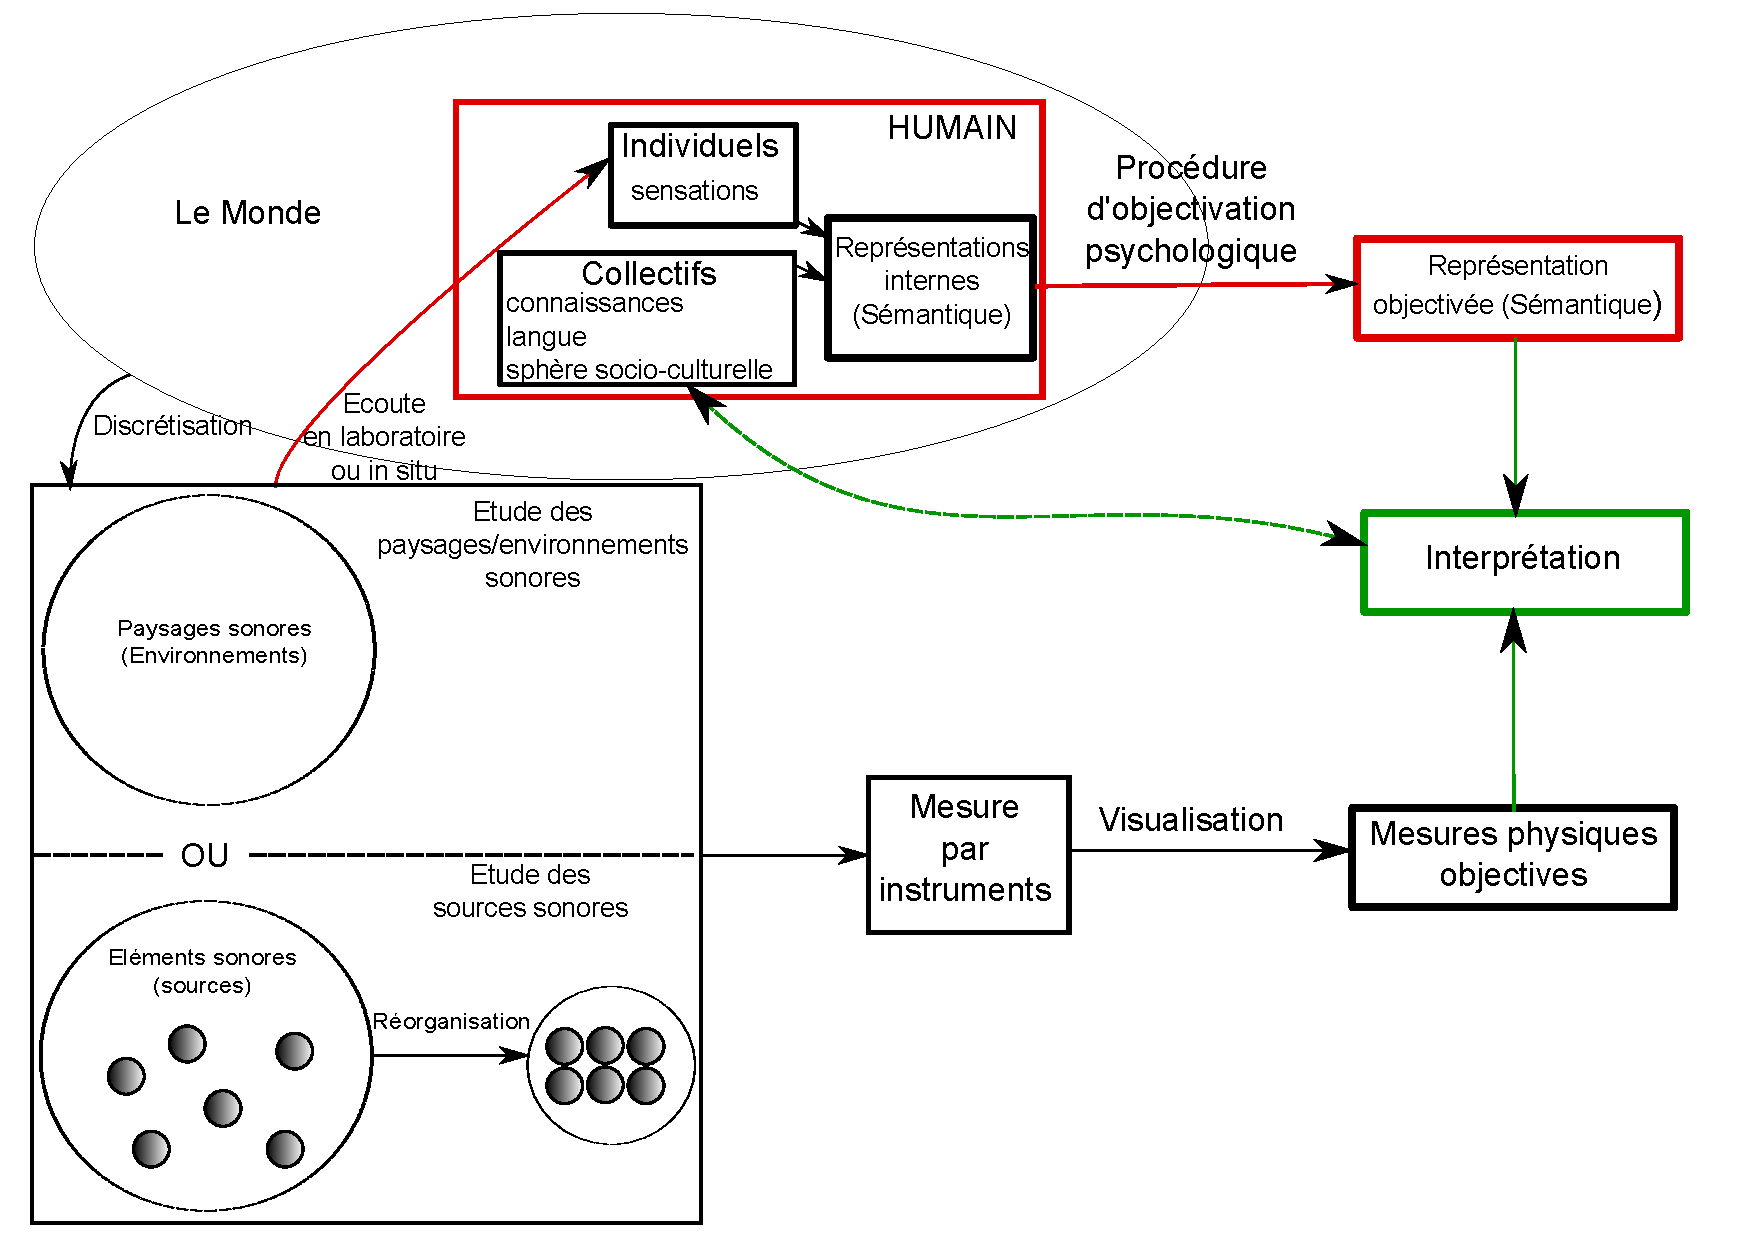
\includegraphics[width=\linewidth]{gfx/Shema_maffiolo}
        \caption[Paradigme du cognitivisme]{Paradigme du cognitivisme, d'après \citep{maffiolo_caracterisation_1999}}\label{fig:paradigmeCognitivisme}
\end{figure}

\subsubsection{L'approche Écologique}
\label{sec:ecologique}

L'approche écologique a d'abord été introduite dans le domaine de la vision par Gibson \citep{gibson1966senses}, qui se demande entre autre si les ``\,lois structurant les objets sont porteuses d'informations, ou si cette information est tirée de comparaison\,'' \citep{gibson1978ecological}.

Cette approche reconnaît que la réponse à un stimulus dépend et de l'information perçue (processus \emph{bottom-up}), et de la connaissance du monde (processus \emph{top-down}), autrement dit l'environnement quotidien et le contexte habituel d'écoute du stimulus.

Afin de garantir une validité écologique, l’approche écologique requiert, dans le cadre d'études perceptives sonores, de prendre en compte cet environnement particulier dans lequel gravitent le sujet et le stimulus. Elle s’oppose ainsi aux méthodes expérimentales traditionnelles, celles de la psychophysique en particulier, en postulant que les expériences en laboratoire décontextualisent le sujet et sa réponse. Une expérience en laboratoire demande en effet au sujet de fournir un effort d'abstraction supplémentaire afin de s’imaginer dans des conditions d'écoute réelle.

A ce titre, un grand nombre d'étude se pratique maintenant dans un cadre \emph{in situ}. On parle d'ailleurs de \emph{soundwalk}  \footnote{\emph{Soundwalk} est un terme anglais introduit par R. Murray Schafer \citep{schafer1969new} signifiant littéralement ``\,marche sonore\,''. Ce terme étant couramment utilisé en français, il ne sera pas traduit dans ce document} pour désigner les expériences où le sujet est immergé dans l'environnement qu'il doit évaluer \citep{adams2008soundwalking,jeon2013soundwalk}.

La méthode des \emph{soundwalk} permet entre autre:

\begin{itemize}
\item  de contextualiser le sujet, à savoir, l'évaluer dans un environnement qu'il connaît et potentiellement qu'il pratique (lieu de vie, de travail)
\item d'évaluer l'environnement sonore, tout en maintenant actif les autres sens (vue, olfaction)
\item de circonvenir aux problèmes de reproduction des environnements sonores en laboratoire
\end{itemize}

Ce problème d'une reproduction écologique des environnements sonores en laboratoire a été particulièrement étudié par Guastavino. \citep{guastavino2003approche,guastavino2004perceptual,guastavino2005ecological}. En comparant les descriptions verbales produites à la suite d'écoutes \emph{in situ} , ainsi que d'écoutes effectuée en laboratoire via des systèmes de reproduction stéréophoniques et multi-phoniques, \citep{guastavino2005ecological} montre que les événements sonores peuplant les scènes sont décrits de la même manière quelque soit le contexte d'écoute. Cependant des différences ont été trouvées concernant la description des fonds sonores (\emph{sound backgrounds}), entre les écoutes stéréophoniques, et les celles multi-phoniques et \emph{in situ}, suggérant de fait que le système de reproduction influe sur les processus cognitifs mis en œuvre. Des conclusions similaires sont faites dans \citep{guastavino2004perceptual} en considérant cette fois-ci des systèmes de reproduction mono, stéréo, et multi-phoniques.

Cependant, les études \emph{in situ}, bien qu'étant écologiquement plus valides que des études en laboratoire, présentent elles aussi des inconvénients. Dans le cas où tous les sujets ne passent pas l'expérience au même moment, il est impossible de garantir qu'ils soient soumis aux mêmes stimuli. De facto, la reproductibilité des expériences est elle aussi plus difficile. A l'inverse, le cas où l'expérience est passée de manière simultanée par tous les sujets peut faire émerger des problèmes pratiques d'organisation, notamment en ce qui concerne le maintien du sujet dans une attitude propice à passer une expérience.

\subsection{L'écoute}

\subsection{Le chaîne traitement de l'information auditive}
\label{sec:chaineTaite}

Le son est une vibration émise par une source d'excitation, et transmise à l'air. Cette vibration se propage ensuite jusqu'à atteindre un récepteur, le tympan, qui va capter le différentiel de pression résultant de cette vibration. C'est le point de départ du processus de traitement de l'information auditive. 

Si on adopte une approche \emph{traitement de l'information}, on peut décomposer ce processus en plusieurs systèmes inter-connectés. Ces systèmes forment une chaîne qui, au fur et à mesure des traitements, interprète le signal acoustique afin d'en extraire l'information sémantique. Plus on se place loin dans la chaîne de traitement, plus on a accès à une information abstraite, potentiellement utilisable par d'autres processus de haut niveau. La figure \ref{fig:traitementSonMcAdamsBigand} extraite de \citep{mcadams1994penser} nous donne un aperçu des principales fonctionnalités du système de traitement auditif.

\begin{figure}[bth]
        \myfloatalign
        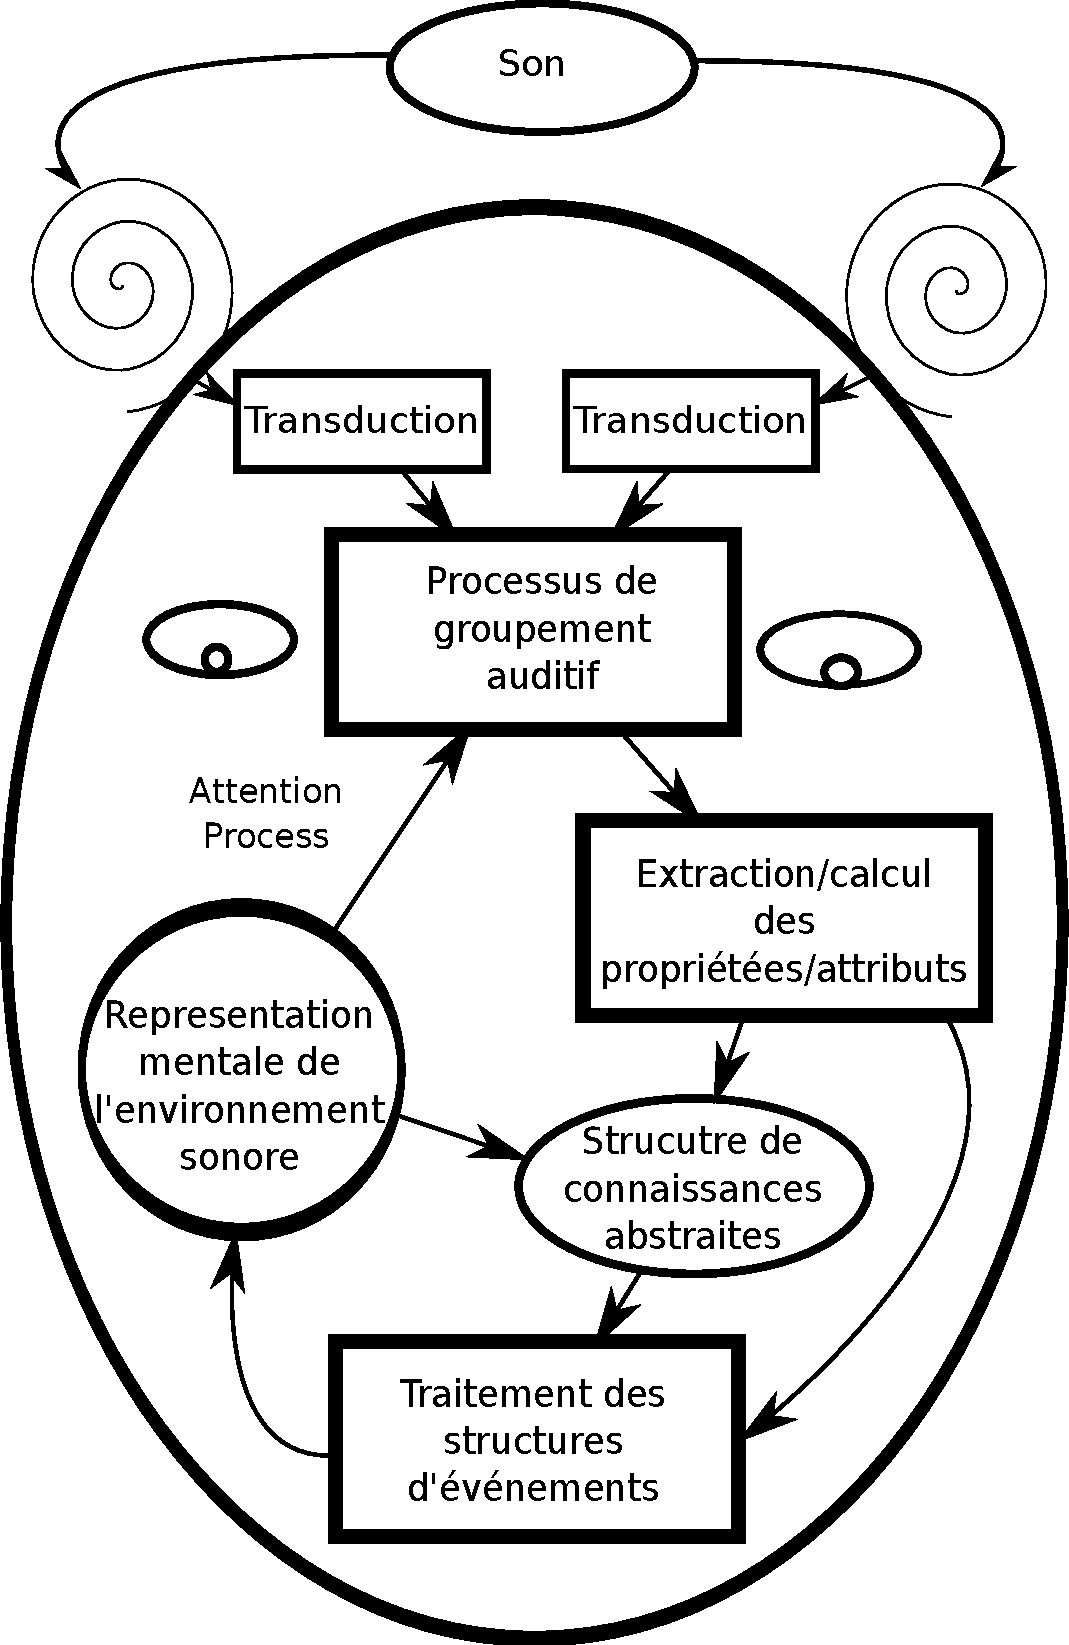
\includegraphics[width=.6\linewidth]{gfx/traitementSonMcAdamsBigand}
        \caption[Principaux processus de traitement de l'information auditive et leurs interactions]{Principaux processus de traitement de l'information auditive et leurs interactions, à partir de \citep{mcadams1994penser}}\label{fig:traitementSonMcAdamsBigand}
\end{figure}

Lors de l'étape de \emph{transduction}, les vibrations sonores parvenant au tympan sont analysées puis traduites en impulsions nerveuses transmises au cerveau. Ces impulsions rendent compte des attributs spectraux et temporels de l'onde. L'extraction des composantes fréquentielles intervient dans la cochlée. C'est à l'intérieur de cette dernière que les différentes parties de la membrane basilaire vont être excitées en fonction des fréquences composant le signal, suivant un axe tonotopique. Les vibrations captées à chaque point d’excitation de la membrane basilaire sont transmises au cerveau via les nerfs auditifs, chaque point codant une information correspondant à une bande fréquentielle limitée. 

Vient ensuite le \emph{processus de groupement auditif}. C'est une étape d'intégration temporelle au cours de laquelle l'information est analysée en images auditives cohérentes. Contrairement à ce que pensaient les Grecs, nous ne possédons pas de "canaux" séparés pour chaque objet sonore présent dans l'environnement \citep{yost1994fundamentals}. C'est notre cerveau qui se charge de fusionner et de discrétiser les éléments sonores simultanés afin de créer un flux auditif structuré. En d'autres termes il s'agit de déterminer, combien d'objets sonores sont présents, d'où viennent t-ils et quel est leur sens. Les recherches regroupées sous l'appellation ``\,analyse de scènes auditives\,'', abordées à la section~\ref{sec:ASA} ont  extensivement étudié ces processus de groupement.

Prenons pour exemple les chorals de Bach. C'est le \emph{processus de groupement auditif} qui nous permet, sur la base des paramètres spectro-temporels du signal, de distinguer les quatre voix basse, ténor, alto et soprano. Par contre c'est à partir d'une analyse des attributs perceptifs que nous sommes capables de percevoir les mélodies comme des objets unitaires, même si ces dernières sont développées entre les différentes voix du choral. Cette extraction des propriétés perceptives intervient pendant la phase dite \emph{d'extraction/calcul des propriétés/attributs}.

Une définition des représentations mentales est donnée par \citep{houde1998vocabulaire}:

\begin{quote}
``\,La représentation mentale peut être vue comme une entité interne, le correspondant cognitif individuel des réalités externes expérimentées par un sujet.\,''
\end{quote}

Ces représentations font office de sauvegardes de l'information. Conservées en mémoire sous une forme hautement abstraite \citep[p. ??]{mcadams1994penser}, elles rendent compte à la fois de notre compréhension du monde et de la manière dont nous l'abordons. Ces connaissances subjectives, non directement observables, restent néanmoins accessibles au chercheur par le biais d'expériences d'objectivation (voir section~\ref{sec:appCategorielle})

\subsection{Processus Bottum-up et processus Top-down}

L'interaction entre l'homme et son environnement est fonction d'une part de l'information sensorielle captée par le sujet, d'autre part de la rétroaction exercée par lui sur ces données. Cette rétroaction est déterminée par son expérience sensible du monde. Par "expérience sensible", nous entendons la mémoire interne des interactions passées, mémoire grâce à laquelle nous optimisons l'analyse des stimuli, et intégrons les effets de contexte dus à l'environnement.

Cette mémoire est à la fois :

\begin{itemize}
\item individuelle : dépendant de notre expérience propre
\item collective : dépendant des connaissances que nous avons acquises sur le monde
\end{itemize}

La rétroaction est l'expression de l'individualité du sujet, individualité qui explique que deux personnes ayant des capacités sensorielles semblables peuvent percevoir différemment un même environnement.

Ainsi la perception mobilise deux formes de traitements :

\begin{itemize}
\item les traitements dits ascendants (bottom-up) dirigés par les données
\item les traitements dits descendants (top-down) dirigés par les concepts ou les représentations
\end{itemize}

Étudier la perception demande de prendre en compte aussi bien l'information externe (processus ascendant) que l'information interne (processus descendant). Réduire la perception à une simple association de sensations ne permet pas de rendre compte de l'éventail des processus cognitifs entrant dans le décodage de l'environnement. Un exemple parlant concret, emprunté au domaine de la vision, est celui du phénomène dit de bi-stabilité, \ie~La faculté, chez un sujet, de voir dans une même image tantôt un canard, tantôt un lapin, autrement dit, de tirer d'un même stimulus deux analyses différentes, mais jamais simultanément (\Cf~Figure\ref{fig:bistabilite}).

Un autre exemple, cette fois dans le domaine de l'audition, nous semble illustrer le caractère dual de la perception. Il est donné par McAdams et Bigand \citep[p. 2]{mcadams1994penser}:

\begin{quote}
``\,...Imaginez vous un instant en pleine forêt amazonienne : vous entendriez exactement les mêmes bruits que le guide qui vous accompagne, mais, étant donné votre manque de connaissance du milieu, vous seriez incapable d'extraire du fond sonore les sons correspondant aux cris de l'iguane, aux singes macaques, aux chants des ouistitis ou aux bruissements des arbres tropicaux. De ce fait vous seriez dans l'incapacité d'attribuer une signification à l'ensemble de la structure sonore, ce qui pourrait être important pour votre survie dans l'environnement.\,''
\end{quote}

\begin{figure}[bth]
        \myfloatalign
        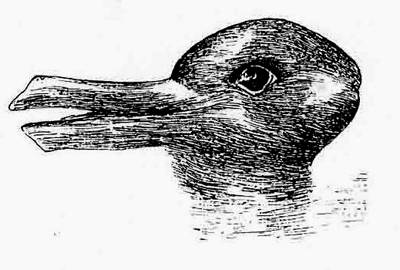
\includegraphics[width=.6\linewidth]{gfx/canard_lapin}
        \caption[Le phénomène de bistabilité: l'illusion du canard-lapin]{Le phénomène de bistabilité: l'illusion du canard-lapin. Première publication dans \emph{Fliegende Blätter}, 23 octobre 1892, p. 147}\label{fig:bistabilite}
\end{figure}

En psychologie cognitive, on distingue ainsi les approches cognitivistes, qui s'intéressent plus particulièrement aux processus de type \emph{botttom-up} relatifs au traitement de l'information perçue , des approches dites cognitives, lesquelles interrogent, avant tout, les processus de type \emph{top-down} liés à la mémoire du sujet ainsi qu'au contexte \citep[p. ??]{guastavino_etude_2003}.

\section{Représentation mentale de l'environnement sonore}
\gl{Cette partie (Représentation de l'environnement sonore) devra être réorganisée. s'appuyer sur \citep{Houix03f} et \citep{goldstone2003concepts}. Ne pas corriger}

Les représentations forment une image mentale discrète d'un monde physique continue \citep{houde1998vocabulaire}. C'est par ce passage du continu au discret que nous sommes à même d'organiser nos connaissances, afin de les réutiliser de manière efficace. Les objets discrets qui forment cette organisation sont appelés des catégories. L'action consistant à juger si un événements perçu appartient à une catégorie, est elle appelée la catégorisation.

\subsection{Théorie de la catégorisation}

Nous considérons ici le processus de catégorisation comme initialement formalisée par E. Rosch et B. B. Lloyd \citep{rosch1978cognition}, et nommée théorie prototypique de la catégorisation. Il est à noter que l'étude de la catégorisation est antérieure aux travaux de Rosch, et que depuis, d'autres proposition ont été faite afin d'étendre la théories prototypique, comme la théories des exemplaires ou \textit{context theory} \citep{medin1978context}, et son extension multidimensionnelle \citep{medin1978context}. Mais les travaux de Rosch étant à l'origine de ces théories postérieures, nous nous appuierons sur ces derniers afin de détailler de manière générale le fonctionnement des processus de catégorisation. 

Un des principes essentiel de tout être vivant est de segmenter son environnement, \ie~de se bâtir un système de classification permettant de regrouper des objets n'étant pas identiques \citep[p. 1]{rosch1978cognition}. On appelle catégorisation, l'action consistant à regrouper des objets du monde physique considérés comme équivalents, et catégorie, l'objet mental contenant le groupe d'objets ainsi rassemblé. 

Il est important de noter qu'à chaque catégorie est associé un label, censé décrire du mieux possible l'ensemble des objets inclus dans la catégorie. On parlera alors de catégories sémantiques. L'ensemble des catégories sémantiques conservées en mémoire forment la représentation mentale qu'un individu se fait du monde, des réalités externes. 

L'introduction de cette dimension sémantique a des conséquences importantes sur l'universalité présupposée de la catégorisation. Cette dernière étant codée par la langue, elle ne dépend plus seulement d'une réalité physique, mais également d'un contexte culturel. La catégorisation peut être vue comme un action intermédiaire entre, d'une part l'organisation d'une connaissance individuelle résultant d'une expérience sensorielle personnelle, et la constitution d'une représentation collective pouvant être partagée par le biais d'un langage commun \citep{dubois2006cognitive}. 

Selon Rosch, la catégorisation obéit à deux principes \citep[p. 29]{rosch1978cognition}:

\begin{enumerate}
\item \textit{L'économie cognitive}: la catégorisation doit fournir un maximum d'information pour un minimum d'effort. La structure du système catégoriel s'élabore en tenant compte de se principe d'économie. On comprend alors que la catégorisation d'un objet est soumise à un contexte sensoriel, c'est à dire aux autres objets perçus simultanément, et qui doivent être eux aussi catégorisés. Comme énoncé par D. Dubois \citep[p. 33]{dubois1991semantique}:
\begin{quote}
``\,Catégoriser un stimulus signifie le considérer dans la finalité de cette catégorisation, non seulement comme équivalent des autres stimuli de la même catégorie, mais également différent des stimuli qui n'appartiennent pas à cette catégorie\,''.
\end{quote}

Il apparaît clairement que la catégorisation d'un objet ne se veut pas absolue, autrement dit, l'appartenance d'un objet à une catégorie ne dépend pas uniquement de l'observation d'une propriété particulière, mais également du contexte dans lequel cette objet est perçu.

\item \textit{La redondance structurelle}: l'ensemble des objets physiques ne vie pas dans un espace aux dimensions bien identifiées, finies, et dont les valeurs seraient équiprobables. En d'autres termes, le monde ne peut se réduire à des paramètres dimensionnés, indépendants et manipulables, comme dans le cadre d'études en laboratoire. Au contraire, il peut exister des discontinuités saillantes entres objets, de même que ces objets sont souvent liés entre eux par des patterns de co-occurrence de propriétés (exemple : un chien possède "quatre pattes et un museau" plus souvent que "deux pattes et un museau"). Ces discontinuités et corrélations, présentes dans les propriétés perçues, étayent la structure catégorielle de notre représentation mentale,  et gouvernent ainsi le processus de catégorisation.
\end{enumerate} 

Rosch propose de voir la structure catégorielle suivant deux axes:

\begin{itemize}
\item \textit{axe vertical}: Il s'agit de l'organisation hiérarchique des catégories, qui illustre la manière dont les catégories sont incluses les unes dans les autres. Cette dimension verticale peut être vue comme une taxonomie, les catégories de haut-niveaux représentant des objets abstraits ou concepts, et incluant un grand nombre de sous catégories, et les catégories de bas-niveaux représentant des objets concrets, incluant peut de sous catégories. Ainsi, plus le niveau d'abstraction est grand, plus les similitudes entre objets d'une même catégorie (intra-catégorielle), ainsi que la similitude entre objets de catégories distinctes (inter-catégorielle) son faibles. Inversement, plus le niveau d'abstraction est faible, plus les similitudes intra- et inter-catégorielle sont élevées. Rosch propose de décomposer cette dimension verticale en trois niveaux d'abstraction (\Cf~Figure~\ref{fig:categorieLVL}): Superordonné, Base et subordonné. Le niveau superordonné représente les catégories avec un haut niveau d'abstraction tandis que le niveau subordonné représente les catégories concrètes. On voit bien que les périmètres définis par les catégories du niveaux superordonnées (Mobilier, Véhicule) sont larges, \ie~les objets contenus dans ces catégories peuvent être très distincts. A contrario, les catégories du niveaux subordonnées (chaise longue, cabriolet) sont très précises, et les objets qu'elles contiennent très similaires entres eux. Cependant, on notera que les objets de la classe Cabriolet ont potentiellement beaucoup de propriétés en commun avec les objets de la classe Berline (par exemple), beaucoup plus que celles que partagées entre les objets des classes Mobilier et Véhicule. 
\item \textit{axe horizontal}: Cette dimension peut être vue de deux manières: 1) elle illustre la manière dont sont séparées des catégories partageant le même niveau d'abstraction, 2) elle permet d'apprécier le degré de typicité des différents objets appartenant à une même catégorie. En effet, les catégories ne sont pas des objets discrets, car les propriétés attribuées aux objets qu'elles contiennent peuvent être partagés par d'autres catégories. Ainsi, les frontières entre les différentes catégories ne sont pas figées et peuvent se recouvrir. Pour discriminer les catégories, Rosch propose de ne pas raisonner en terme de frontières, mais plutôt de décrire chaque catégorie par un nombre de cas non ambiguës (clear case) \citep[p. 36]{rosch1978cognition}. Tous les objets d'une catégorie ne sont pas également représentatifs de cette dernière, les cas non ambiguës peuvent être vus comme les objets les plus typiques de la catégorie. Ce fait est empirique, il a été montré que des sujets peuvent très bien s'accorder sur la typicité d'un objet par rapport à une catégorie, tout en n'étant pas d'accord sur les frontières de cette dernière \citep{rosch1974human,rosch1975cognitive}. Le terme prototype, qui donne son nom à la théorie, vient de l'hypothèse que, parmi ces cas non ambiguës, il en existe un, le prototype, plus représentatif que les autres, et qui forme le noyau de la catégorie.
\end{itemize}

\begin{figure}[bth]
        \myfloatalign
        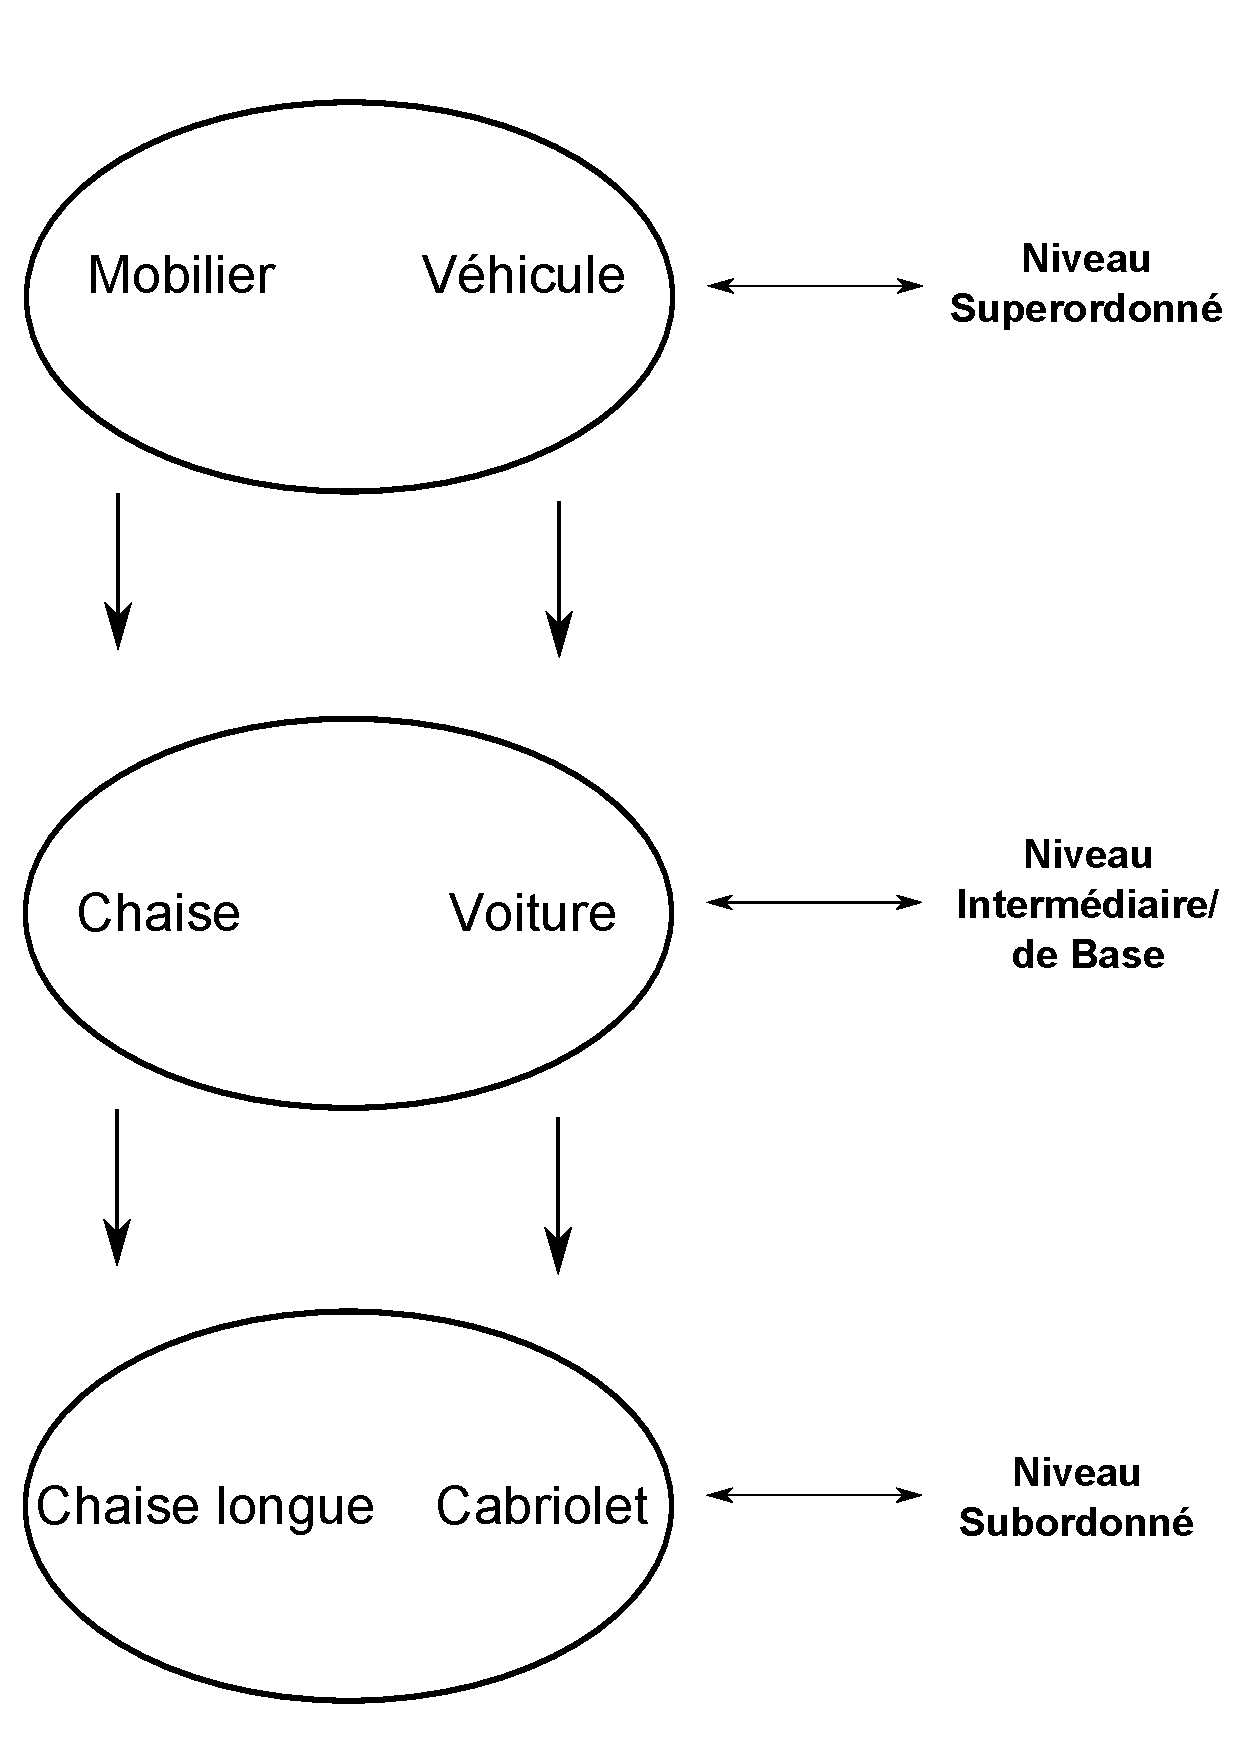
\includegraphics[width=.6\linewidth]{gfx/categorieLVL}
        \caption{Les trois niveaux d'abstraction de l'axe vertical de la structure catégorielle.}\label{fig:categorieLVL}
\end{figure}

Les catégories sont structurées en interne, en référence à un prototype, \ie~l'objet possédant les attributs typiques de celle-ci. L'appartenance d'un objet à une catégorie dépend alors de la ressemblance qu'entretient ce dernier avec le prototype.  Plusieurs proposition ont été faites afin de définir le prototype d'une catégorie: Pour Tversky \citep{tversky1977features}, le membre prototype sont celui dont la somme des similarités avec les autres membres de la catégorie est la plus grande. Pour \citep{rosch1975family}, il s'agit de l'objet possédant le plus de propriétés en commun avec les objets de la catégorie, et le moins de propriétés avec les objets des catégories externes. Dans ce cas, la typicité d'un élément d'une catégorie est donc fonction de son degré d'appartenance à celle-ci, ainsi que de son indépendance vis à vis des autres catégories. En se limitant à l'observation d'attributs vivant dans un espace métrique, \citep{reed1972pattern, rosch1976structural} ont montré que le prototype est un centroid, un objet définit comme étant la moyenne des attributs des objets de la catégories.

Mais il faut bien comprendre que cette théorie prototypique de la catégorisation, bien que se basant sur des faits expérimentaux, est avant tout une vision pratique, un concept qui n'a pas été clairement défini et dont l'implication dans les processus de catégorisation reste floue \citep[p. 36-40]{rosch1978cognition} \citep[p. 49-54]{dubois1991semantique}.

\section{Analyse de scènes acoustiques}
\label{sec:ASA}

\subsection{Définition}
\label{sec:ASAintro}

L'analyse de scène est un terme d'abord introduit de la cadre des recherches informatiques en vision. Il fait référence aux différentes stratégies par laquelle un ordinateur parvient à isoler un objet d'une image~\citep[p. 12]{mcadams1994penser}. Le pendant acoustique de l'analyse scène, est nommé l'Analyse de Scène Acoustique (ASA). Le terme ASA a été introduit par Albert S. Bregman dans son ouvrage de référence \citep{bregman1994auditory}.  

L'ASA désigne l'ensemble des processus perceptifs permettant d'isoler d'une mixture sonore \footnote{On entend par mixture sonore, ou magma sonore, un ensemble de sons provenant de différentes sources sonores}, les informations émanant d'une source sonore distincte, et à les regrouper afin de les traiter comme un tout cohérent.  L'ASA part en effet du principe que, afin de faire sens de l'environnement qui l'entour, il est nécessaire pour le cerveau d'isoler les informations relatives aux différentes sources sonores \citep{winkler2009modeling}. On parle alors indifféremment de processus de ségrégation ou de groupement.

La définition de l'ASA est très large. Comme vu dans la section~\ref{sec:chaineTaite}, les processus de groupement sont composés à la fois de processus \emph{bottum-up}, \ie~ dirigés par l'information auditive transduite (représentation temps-fréquence du signal sonore), ainsi que de processus \emph{top-down} dirigés par les connaissances stockées en mémoire. Dans la théorie de l'ASA, les processus \emph{bottum-up} sont appelés \emph{processus primitifs}, et les processus  \emph{top-down}, \emph{processus basés sur des schémas}. 

Pour les premiers, il s'agit de systèmes de traitement innés, opérant sur la base de régularités présentes dans le signal, afin de regrouper les composantes fréquentielles produites par une même source. Par régularité on comprend ici des propriétés constantes de l'environnement, perçues par l'ensemble des êtres humains, partout sur la planète. Par exemple, si la fréquence fondamentale d'un son harmonique change au cours du temps, toutes ses harmoniques changeront également afin de maintenir la structure harmonique du son [p. 38]\citep{bregman1994auditory}. Les \emph{processus basés sur des schémas}  partent eux de schémas, \ie~connaissances apprises formant notre représentation mentale du monde, formés par le biais d'écoutes antérieures. 

La plupart des recherches sur l'ASA adopte encore maintenant une approche cognitive, en se concentrant sur l'étude des \emph{processus primitifs}. Cependant, elles suivent généralement une méthodologie expérimentale très inspirée de la psychoacoustique.

\subsection{Une approche psychoacoustique}

L'étude de l'ASA adopte une méthodologie s'inspirant largement du paradigme de la psychoacoustique. Ainsi les réponses du sujets sont évaluées par rapport à un stimuli décrit analytiquement dans un espace multidimensionnel de dimensions physiques (fréquence, intensité etc $\ldots$) \citep{dubois2006cognitive}. Dans la grande majorité des cas, les stimuli utilisés sont des sons pures ou complexes\footnote{Par son pur on entend un son composé d'une seule sinusoïde, \ie~possédant une seule fréquence. A contrario, un son complexe est un son composé de plusieurs composantes fréquentielles}, bien évidemment synthétisés en laboratoire. 

Ces sons sont alors proposés à l'écoute à un sujet, de manière séquentielle. Il s'agit alors, au cours de la séquence, de faire varier un paramètre (intensité, hauteur fréquentielle, espacement entre les séquences), et d'observer le seuil à partir duquel ce changement a un effet significatif sur la capacité du sujet à distinguer plusieurs sources sonores.

L'étude de l'ASA se restreint donc à l'analyse de l'effet de descripteurs bas niveaux sur les processus d'intégrations, sans tenir compte d'attributs perceptifs plus haut niveaux, comme la valeur sémantique attribuée aux sons, ni de considérations écologiques~\ref{sec:ecologique}. En conséquence, il est parfois difficile de faire le lien entre la notion de source sonore comme utilisée dans les études psychoacoustique de l'ASA, et celle adoptée par les études en psychologie cognitive. En théorie, pour les deux approches, le terme source sonore se réfère directement à l'objet (\eg~voiture) supposé être la source d'émission d'un son réel. En psychologie cognitive, cette relation est directe, le stimuli étant la plupart du temps un enregistrement de ladite source. En psychoacoustique, la relation directe est difficile, les stimuli étant des sons de synthèses, inexistant dans le monde réel. La source sonore désigne alors plutôt un objet abstrait, dont l’existence est avérée à partir du moment ou un agglomérat de sinusoïdes est interprété par le sujet comme étant un tout, émanant de facto d'une seule entité. 

Il s'agit là d'une des limitations de l'approche psychoacoustique appliquées aux études des  \emph{processus primitifs} de l'ASA. Les résultats, obtenus à partir de stimuli très éloignés de la réalité des phénomènes acoustiques perçus, étant difficiles à généraliser à des applications plus incarnés.

\subsection{Régularités et processus primitifs}

L'existence des \emph{processus primitifs} est une conséquence de la présence dans le monde sonore de régularités universelles affectant l'ensemble des stimuli auditifs. Bregman distingue 4 types de régularités [p. 19,21,31,33]\citep{mcadams1994penser}:

\begin{enumerate}
\item \emph{Synchronicité}: Il est rare que des sons n'ayant aucun rapport entre eux démarrent et s'arrêtent au même moment.
\item \emph{Continuité}: 
\begin{itemize}
\item Les propriétés d'un son isolé tendent à se modifier lentement et de façon continue.
\item Les propriétés d'une séquence de sons émis par la même source tendent à se modifier lentement.
\end{itemize}
\item \emph{Harmonicité}: Lorsqu'un corps sonore vibre à une période répétée, ses vibrations donnent naissance à un pattern acoustique dont les fréquences des composants sont des multiples d'une même fréquence fondamentale
\item \emph{Uniformité}: La plupart des modifications qui surviennent dans un signal acoustique affectent tous les composants du son résultant, de manière identique et simultanée.
\end{enumerate}

Notre perception du monde est contrainte par la présence de ces régularités. A ce titre, les \emph{processus primitifs} sont des systèmes perceptifs innés, uniquement dépendant des stimuli. On peut les voir comme une série de règles génériques qui nous permettent, sur la base des régularités, d'isoler du monde sonore des objets cohérents \citep{ballas1987interpreting}. Il s'avère que ces règles sont très proches de celles opérant pour la perception des formes dans le cadre de la vision.  

\subsection{Perception de la forme}

Que ce soit en vision ou en audition, notre cerveau est en permanence stimulé un ensemble de sources distinctes. Percevoir un objet dans cet agglomérat, c'est être capable d'isoler tous les signaux émis par une même source, et de les réunir en une unité perceptive cohérente.

Parmi les premiers travaux qui se sont intéressés à ces processus de groupement, on trouve la psychologie de la forme, ou plus communément appelée \emph{Gestalt Theory} (\emph{Gestalt} étant un mot allemand pouvant être traduit par forme). Cette théorie, introduite par Ernst Mach et Christian von Ehrenfels à la fin du XIXème siècle, se propose d'expliciter les principes selon lesquels des stimuli sensoriels sont combinés afin de former un pattern mental rendant compte de la présence d'un objet présent dans l'environnement. 

Ces principes ont principalement été établis en considérant le problème de la perception visuelle. Mais il a depuis été montré qu'ils restent vrais dans le cadre de la perception auditive \citep[ch. 1]{bregman1994auditory}. Parmi ces principes, nous en détaillons cinq:

\begin{enumerate}
\item \emph{Proximité}: Des éléments proches les uns des autres ont tendance à être groupés ensembles. En audition, ce principe de proximité opère suivant les différentes caractéristiques du sons, à savoir, la fréquence, l’onset \footnote{En traitement du signal audio, on désigne par le mot anglais onset le début du signal. Ce terme étant couramment utilisé en français, nous ne le traduirons pas dans ce document.} et l'intensité. 
\item \emph{Similarité}: Des éléments qui se ressemblent ont tendance à être groupés ensembles.
Dans le domaine de la vision, la proximité est réservée au domaine spatial, alors que la similarité est réservée aux caractéristiques physiques de l'objet (forme, couleur, etc $\ldots$), qui ne peuvent se décrire suivant une unique dimension. De même en audition, on parlera de manière générale de proximité temporelle (onsets proches) et non de similarité. Pour le reste des descripteurs utilisé en audition, il est cependant difficile de clairement distinguer les principes de proximité et de similarité. Bregman propose de réserver le terme proximité lorsque l'on considère une dimension physique particulière, et d'utiliser le terme similarité lorsque l'on considère un ensemble de descripteurs, ou lorsque l'on traite d'attributs qui ne peuvent être clairement décomposés suivant des dimensions distinctes, comme le timbre.
\item \emph{Continuité}: Des éléments qui varient de manière non abrupte ont tendance à être groupés ensembles. Par ce principe, des objets distincts mais proches temporellement (respectivement spatialement pour la vision) ont tendance à être perçus comme le prolongement des uns par rapport aux autres. A contrario, une changement abrupte indique généralement l'apparition d'une nouvelle source. C'est ce principe qui nous permet de percevoir comme une seule entité, un objet dont les caractéristiques varient dans le temps,\eg~le son d'une sirène.
De récentes études en neurosciences ont montré l'importance de ce principe dans les processus de groupement. Notamment\citep{winkler2009modeling} qui proposent de voir l'ASA comme un processus prédictif, le cerveau cherchant à anticiper la nature des stimuli qui lui parviennent, sur la base de régularités extraites des objets détectés dans l'instant précédant.
\item \emph{Clôture}: Des éléments discontinus qui suggèrent la forme d'un objet continu ont tendance à être groupés ensembles. De manière automatique, le cerveau tend à percevoir un ensemble d'objets distincts comme un tout. En audition, ce principe est très lié à la notion de masquage. En effet, les sons que nous percevons sont régulièrement masqués par d'autres sons concurrents, potentiellement beaucoup plus fort. Le principe de clôture nous permet de compenser ce phénomène de masquage et de percevoir le signal sans discontinuité. Ainsi lorsqu'un son pure est régulièrement entrecoupé de silence, nous percevons une série de sons pures, mais, si les silences sont comblés par un bruit blanc, nous percevons un son pure continue. Ce phénomène est parfois appelé ``\,l’illusion de continuité\,'' \citep{dannenbring1976perceived}, et s'applique particulièrement dans le contexte de la perception de la parole \citep{carlyon2002continuity}.
\item \emph{Destin commun}: Des éléments qui varient de manière synchrone et uniforme ont tendance à être groupés ensembles. Comme évoqué à la section~\ref{sec:ASAintro} c'est ce principe qui permet de percevoir comme un tout les différentes harmoniques qui composent un son complexe. C'est également ce principe qui nous incite à percevoir de manière unie des stimuli ayant le même onset temporel.
\end{enumerate}

Ces principes agissent de concert afin de grouper les composantes du sons en flux auditifs.

\subsection{Flux auditif et stratégie de groupement}

\begin{figure}[bth]
        \myfloatalign
        \subfloat[]
        {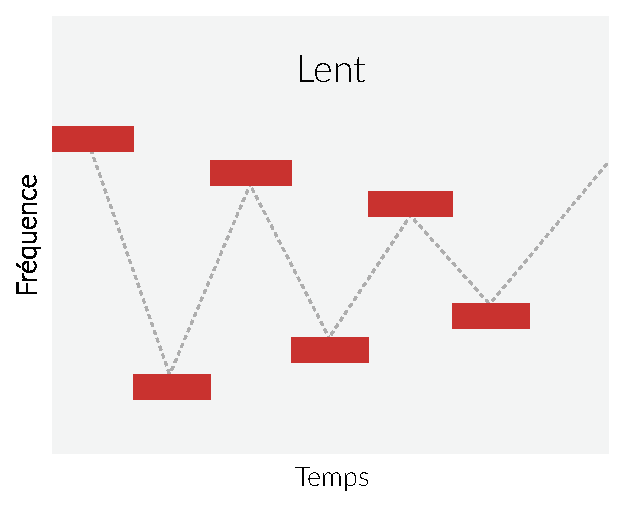
\includegraphics[width=.5\linewidth]{gfx/tonesim_slow}}
        \subfloat[]
        {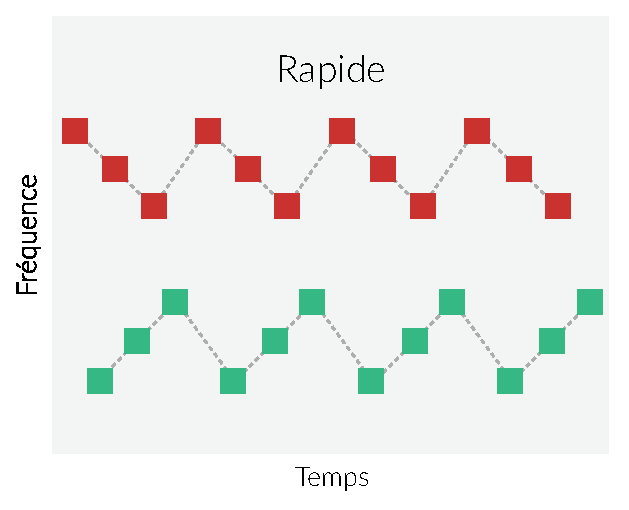
\includegraphics[width=.5\linewidth]{gfx/tonesim_fast}}
        \caption[Groupement séquentiel : proximité temporelle.]{Groupement séquentielle: proximité temporelle. Dans l'exemple (a), la durée entre les événements est telle qu'aucun groupement n'est effectué, les sons sont perçus comme des événements distincts. Dans l'exmple (b) la durée entre les événements est réduite et un groupement s'opère suivant la proximité fréquentielle. Deux flux sont ainsi crées, le premier (rouge) regroupe les sons haute fréquence, et le deuxième (vert) les sons basse fréquence.}\label{fig:tonesim}
\end{figure}

\begin{figure}[bth]
        \myfloatalign
        \subfloat[]
        {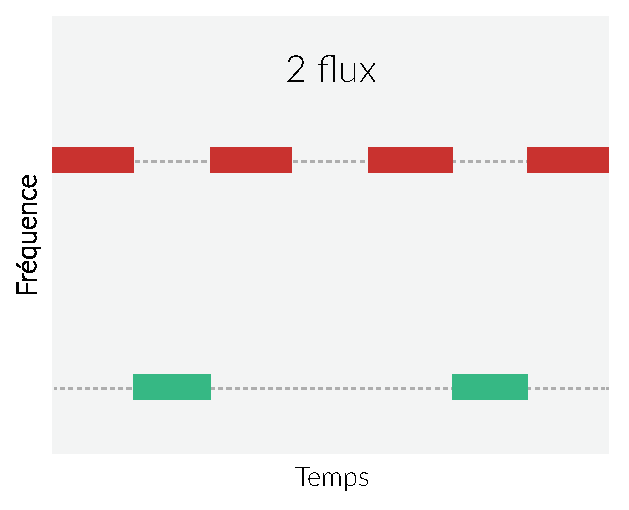
\includegraphics[width=.5\linewidth]{gfx/gallop_2flux}}
        \subfloat[]
        {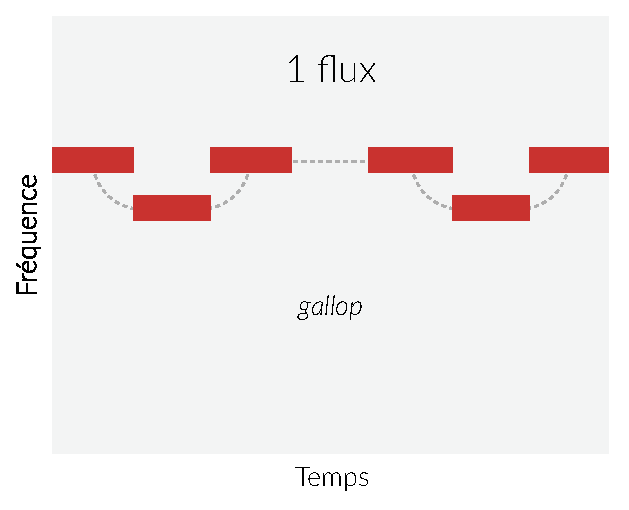
\includegraphics[width=.5\linewidth]{gfx/gallop_1flux}}
        \caption[Groupement séquentiel : proximité fréquentielle.]{Groupement séquentielle: la proximité fréquentielle. Deux groupes de sons sont joués à deux fréquences. Dans l'exemple (a), la distance entre les fréquences des sons est telle que deux flux sont crées, le premier (rouge) regroupe les sons haute fréquence, et le deuxième (vert) les sons basse fréquence. Dans l'exemple (b) la distance entre les fréquences est réduite et un groupement s'opère suivant la proximité fréquentielle. Un seul flux est crée, et l'on perçoit un pattern temporel rappelant le gallop d'un cheval.}\label{fig:gallop}
\end{figure}

\begin{figure}[bth]
        \myfloatalign
        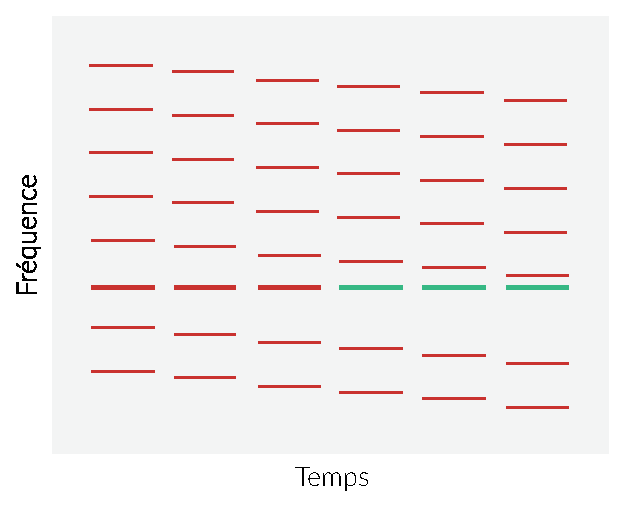
\includegraphics[width=.5\linewidth]{gfx/harmo}
        \caption[Groupement simultané : régularité harmonique]{Groupement simultané : régularité harmonique. Un son complexe est joué plusieurs fois. A chaque occurence, on abaisse les hauteurs de la fréquence fondamentales et des harmoniques de manirèe uniforme. Une harmonique est conservée à fréquence constante (trait gras). Au débur, un flux est crée, \ie~les harminiques et la fréquence fondamentale sont perçus comme étant un seul objet. Au fur et à mesure que la régularité harmonique est brisée, le cerveau tend à percevoir l'harmonique à fréquence constante dans un flux séparé, \ie~comme étant un second objet.}\label{fig:harmo}
\end{figure}

\begin{figure}[bth]
        \myfloatalign
        \subfloat[]
        {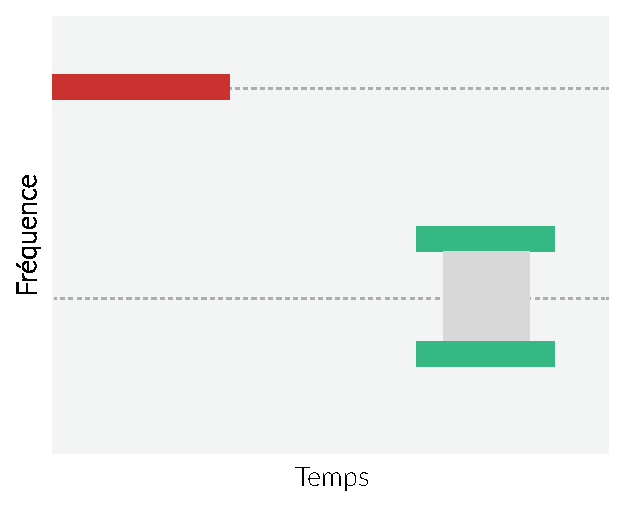
\includegraphics[width=.5\linewidth]{gfx/opn1}}
        \subfloat[]
        {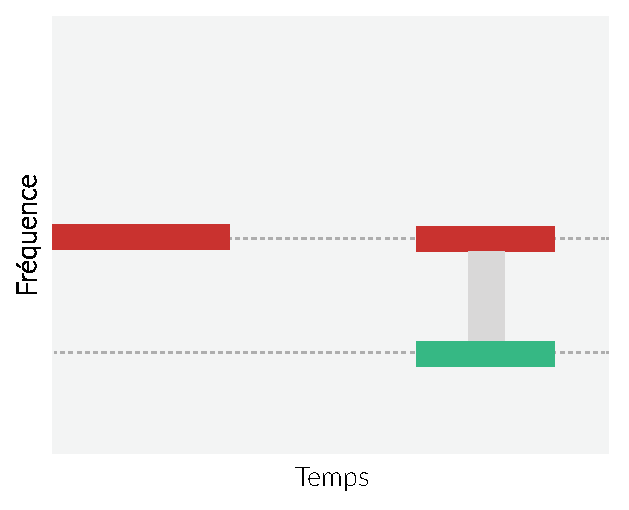
\includegraphics[width=.5\linewidth]{gfx/opn2}}
        \caption[Groupement ancien-plus-nouveau]{Groupement ancien-plus-nouveau. Dans l'exemple (a), les sons A et B ont des fréquences éloignées. Le cerveau génère deux flux, le premier relatif au son A (rouge), et le deuxième comprenant les sons B et C (vert). Dans l'exemple (b), les sons A et B ont la même fréquence. Le cerveau interprète le son B comme étant une continuité du son A. L'attraction entre B et C en est réduite. Le cerveau génère toujours deux flux, le premier regoupant cette fois ci les sons A et B (rouge), et le deuxième le son C (vert).}\label{fig:oldplusnew}
\end{figure}

L'une des notions les plus importante en ASA est le concept de flux auditif (\emph{auditory stream}), que Bregman définit comme ``\,le groupement perceptif que nous faisons des parties du spectre qui vont ensembles\,''.

Contrairement au terme ``\,son\,'', qui peut faire référence tantôt aux réalités physiques des phénomènes acoustiques, aussi bien qu'aux représentations mentales que nous nous en faisons, le flux auditif désigne spécifiquement une entité perceptive.

Le terme flux se veut volontairement généraliste. Ce dernier peut désigner aussi bien un son isolé (un coup de marteau), comme plusieurs sons à condition que ces derniers soient perçus comme formant une seule entité (une série rapprochée de coup de marteau).

On désigne par ``\,formation de flux auditive\,'' (\emph{auditory streaming}) , le processus à l'origine de la création de flux. \citep{winkler2009modeling} propose la définition suivante en ce qui concerne la formation de flux auditif:

\begin{quote}
``\, Un phénomène perceptif dans lequel une séquence de sons est perçue comme étant composée de deux ou plusieurs flux auditifs \,''
\end{quote}

Comme nous venons de le voir, le flux désigne une représentation perceptive d'un son, et à ce titre, il est l'équivalent auditif de l'objet pour la vision \citep[p. 11]{bregman1994auditory}. Cependant, nous notons que la notion de flux, et plus particulièrement la notion de formation de flux, est souvent utilisée dans un contexte ou une dimension temporelle est sollicitée. On parle d'ailleurs de construction de flux  (\emph{build-up of streaming}) pour désigner la période durant laquelle le cerveau accumule des indices afin de générer et stabiliser les flux auditifs  \citep{cusack2004effects,snyder2007toward}. Ainsi dans ce document, nous réservons les termes de flux pour désigner les représentations mentales des stimuli en train d'être traités (intégrés temporellement), de formation de flux auditifs pour désigner les processus perceptives de groupement des sons, mais conservons le terme objet pour désigner de manière générale les représentations mentales stockées en mémoire des phénomènes acoustiques.

Considérant les processus primitifs, on distingue trois stratégies de groupement.

\begin{itemize}
\item \emph{groupement séquentiel}: qui désigne le groupement de sons ne partageant pas un même onset. Dans le cas de sons pures, le groupement séquentiel s'appuie beaucoup sur le principe de \emph{proximité}. Pour des sons pures, il s'agit en particulier de la \emph{proximité} fréquentielle, qui veut que plus deux sons sont proches en fréquence, plus ils auront tendance à être regroupés dans le même flux (\Cf~Figure~\ref{fig:gallop}). Pour des sons complexes, c'est plutôt le principe de similarité qui entre en jeux. La \emph{proximité} temporelle, \ie~la durée séparant chaque son, rentre aussi en ligne de compte. Plus cette dernière est faible, plus deux sons auront des chances d'êtres regroupés (\Cf~Figure~\ref{fig:tonesim}).
\item \emph{groupement simultané}: aussi appelé groupement spectral, il désigne le groupement des composantes fréquentielles qui partagent un même onset. Il s'appuie principalement sur la régularité harmonique. Une composante fréquentielle venant briser la suite harmonique tend à être isolée dans un autre flux auditif (\Cf~Figure~\ref{fig:harmo}).
\item \emph{groupement ancien-plus-nouveau}: Cette stratégie est l'application directe du principe de continuité. Lorsque le spectre de l'environnement sonore s’enrichit subitement tout en conservant ses composantes fréquentielles de départ, le cerveau tend à interpréter l'ajout comme une continuation de l'ancien, et à l'intégrer dans le même flux sonore (\Cf~Figure~\ref{fig:oldplusnew}).
\end{itemize}

Dans le cas d'une compétition entre un groupement séquentiel et un groupement simultané, c'est l'organisation issue du groupement séquentiel qui prime (\Cf~Figure~\ref{fig:simvsseq}). Ce phénomène fait sens d'un point de vu écologique. En effet la plupart des sons, et en particulier ceux utilisés pour la communication, n'existent que dans une certaine durée, et sont intermittents. Il est alors nécessaire de faire des associations entre des sons parfois séparés par un intervalle de temps long afin de percevoir le sens du message. \citep{winkler2009modeling}

Les exemples cités plus haut se placent tous dans un contexte \emph{bottom-up}, en évacuant d'éventuels processus attentionnels. Bien que cela ait été encore très peu étudié, il parait cependant évident que ces stratégies de groupement s’opèrent également  dans un contexte \emph{top-down}, en s'appuyant sur une mémoire à plus long terme.

\begin{figure}[bth]
        \myfloatalign
        \subfloat[]
        {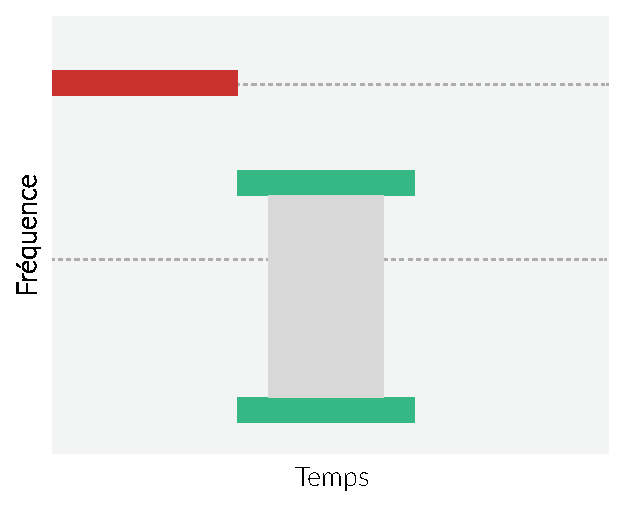
\includegraphics[width=.5\linewidth]{gfx/seqsim1}}
        \subfloat[]
        {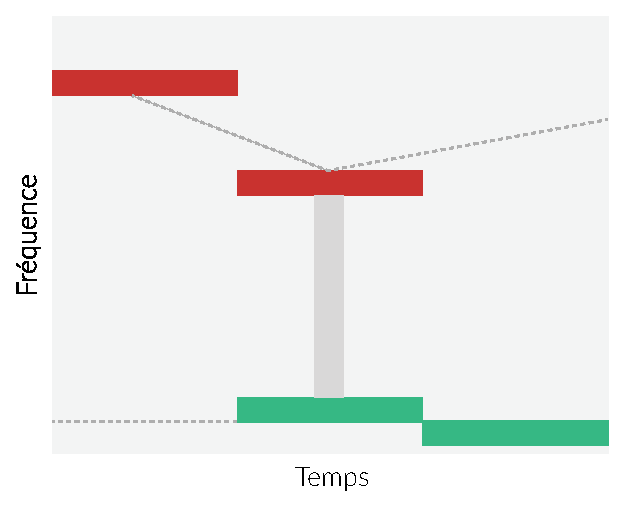
\includegraphics[width=.5\linewidth]{gfx/seqsim2}}
        \caption[Compétition entre groupements séquentiel et simultané]{Compétition entre groupements séquentiel et simultané. Dans l'exemple (a), le cerveau perçoit deux flux, le premier regroupant le son A (rouge) et le deuxième regroupant le sons B et C (vert). Dans l'exemple (b), un quatrième son (D) est ajouté, ce dernier possédant une fréquence très proche de celle de (D). Le groupement sequentiel par proximité fréquentielle entre les couples A-B et C-D est favorisé au détriment du groupement simultané entre les sons B-C.}\label{fig:simvsseq}
\end{figure}



\subsection{Attention et perception}

\subsection{L'approche par les neurosciences}

\section{Le paysage sonore}
\label{sec:paysageSonore}

\subsection{La notion de paysage sonore}

La notion de paysage sonore a été introduite par Schafer dans les années soixante-dix
dans son livre \citep{schafer1969new} et détaillée dans l'ouvrage de référence \citep{schafer1977tuning}. La question que se pose Schafer est alors:

\begin{quote}
``\,Quelle est la relation entre l'homme et les sons de l'environnement qui est le sien, et que se produit-il lorsque ces sons viennent à changer ?\,''
\end{quote}

Bien qu'il n'existe pas de définition consensuelle d'un paysage sonore, la communauté de recherche semble s'accorder \citep{niessen2010categories,aletta2016soundscape} sur celle donnée par B. Truax \citep{truax1978handbook}:

\begin{quote}
``\,Un environnement sonore tel qu'il est perçu et compris par un individu ou une société.\,'' \footnote{Cette définition a été publiée dans le cadre de la norme ISO 12913 \citep{iso12913}}
\end{quote}

La définition se veut très générale. Tout environnement peut être considéré comme un paysage sonore si tant est qu'on lui associe un ensemble de sons entendu par un sujet donné. Le point capital est d'envisager l’environnement sonore par rapport à l'évaluation subjective de l'auditeur, plutôt que de ne prendre en compte que ses paramètres acoustiques. Schafer explicitait déjà la nécessité de ne plus considérer seulement le bruit, mais également sa perception par les individus qui le subissent ainsi que son contexte dans d'écoute, et ce afin de pouvoir améliorer la qualité de l'environnement.

Ainsi, les études sur les paysages sonores suivent le paradigme de la psychologie cognitive \citep{dubois2006cognitive,maffiolo_caracterisation_1999} (voir~\ref{sec:psychoCog}). L'environnement sonore est décrit en utilisant à la fois des descripteurs acoustiques (mesures), ainsi que des descripteurs perceptifs, l'analyse de l'interaction entre ces descripteurs permettant de comprendre les processus cognitifs mis en œuvre dans l'évaluation perceptive des paysages sonores.

L'approche étant ainsi centrée sur le sujet, les recherches sur les paysages sonores sont par essence interdisciplinaires \citep{davies2013perception,aletta2016soundscape}, faisant appel à des outils et méthodes provenant de champs de recherches variés comme l'acoustique, la psychologie cognitive, la psycho-linguistique, la sociologie, et plus récemment, l’intelligence artificielle.

\subsection{Application à la nuisance sonore urbaine}

La ville a toujours été un environnement bruyant, et ce quelles que soient les époques. Ce qui a par contre évolué, c'est la perception de ce bruit. C'est dans les années 80 que l'association bruit/pollution se fait la plus forte. Le bruit est alors considéré comme une dégradation globale de la qualité de vie. En réponse, les recherches sur les environnements sonores se concentrent sur l'identification des sons responsable du bruit, et sur les moyens permettant d'abaisser leurs niveaux sonores. Plusieurs législations anti-bruit sont ainsi mises en place, la grande majorité ayant pour but de combattre les nuisances sonores en réduisant hauts niveaux d'intensité des sons émis par l'industrie ou les transports.

Mais le problème persiste, et pour cause, le bruit demeure un phénomène subjectif, autrement dit dépendant de l'appréciation l'auditeur. Le bruit est affaire de contexte. Le son d'une sirène peut ainsi agacer comme prévenir d'un danger, et beaucoup de quartiers urbains sont appréciés entre autre grâce à leur atmosphère vivante et festive, qui se traduit souvent par des niveaux sonores élevés. Rappelons d'ailleurs que ville agréable, ne rime pas avec ville silencieuse.  


Corriger l'environnement sonore uniquement suivant des paramètres acoustiques, par définition objectifs (par exemple le niveau sonore), ne suffit donc pas. C'est d'ailleurs maintenant largement accepté que des mesures acoustiques objectives, comme le $L_{Aeq}$ ne peuvent rendre compte seules du confort acoustique \citep{yang2005acoustic,schulte2006soundscape,kang2010semantic,aletta2016soundscape}. Afin d'aller plus loin, il faut envisager le bruit comme un objet cognitif, et non comme un objet physique \citep{guastavino_etude_2003}. Il ne s'agit plus de savoir à partir de quand le bruit n'est plus nuisant, mais pourquoi tel bruit est perçu comme gênant par tel individu. Les recherches sur les environnements sonores urbains se sont ainsi tournées vers la notion de paysage sonore, cette dernière envisageant la nuisance sonore d'une manière plus large, prenant en compte les aspects qualitatifs et sémantiques des phénomènes acoustiques. 

De plus, si beaucoup d’effort sont faits afin de réguler les niveaux bruits des sons non-désirés,  l'approche inverse, \ie~ ajouter des sons positivement connotés reste très peu considérée. Cette approche, consistant à identifier et agir sur les sons acceptés ou plaisants afin d'améliorer la qualité d'un environnement, est nommée l'approche positive par Schafer. De récentes études ont montré des résultats prometteurs, notamment \citep{hong2013designing} qui montre que l'ajout de sons d'oiseaux ou d'eau à des sons de trafics urbain permet de significativement améliorer l'appréciation de ces derniers.

Depuis 20 ans qu'elle existe, l'approche par les paysages sonores a déjà permis de développer une base de descripteurs qualitatifs et acoustiques grâce auxquels nous jugeons mieux, et sommes mieux à même d'améliorer l'environnement sonore urbain  \citep{kang2006urban,schulte2007soundscape}

Un des enjeux présent de l'analyse des paysages sonores est de relier ces données perceptives, établies à partir d'enquêtes, à des mesures acoustiques, afin de pouvoir établir une politique de réduction du bruit efficace, adaptée à chaque situation \citep{schulte2013soundscape}.
Cependant, le caractère multi-disciplinaire de ces recherches, et l'utilisation de protocole expérimentaux variés pour évaluer l'environnement sonore, rendent l’intégration des résultats difficile \citep{davies2013perception}. De plus, il n'y a toujours pas de consensus sur les descripteurs (acoustiques ou perceptifs) à utiliser pour caractériser un paysage sonore \citep{brocolini2012prediction,aletta2016soundscape}, empêchant la communauté de proposer aux décideurs en matière de politique d'urbanisation, des indicateurs génériques et clairs, ou des modèles, permettant de rendre compte de la qualité d'un paysage sonore.

Récemment plusieurs projets internationaux ont été lancés afin de standardiser les pratiques expérimentales des recherches s’intéressant aux paysages sonores, notamment \emph{ the European Cooperation in Science and Technology Action}\footnote{TD0804, \emph{soundscape of European Cities and Landscapes}: \url{http://www.cost.eu/COST_Actions/tud/TD0804}} \citep{schulte2010soundscape} et \emph{the Positive Soundscape project} \citep{salford2106,davies2013perception}, mais ces problèmes restent à ce jour ouverts \citep{schulte2013soundscape,ribeiro2013heart}.

\subsection{Objectifs et méthodologie}

\gl{se baser sur \citep{aletta2016soundscape}, définir les objectifs. Introduire les deux approches méthodologiques}

\subsubsection{L'approche catégorielle}
\label{sec:appCategorielle}

Les objectifs de l'approche catégorielle sont triples. Il s'agit 

\begin{itemize}
\item d'appréhender les principes psychologiques qui sous-tendent la formation des représentations mentales
\item d'objectiver la nature de ces représentations
\item de comprendre l'influence de ces représentations sur le traitement de l'information sonore
\end{itemize}
 
A ce titre, l'approche catégorielle peut être vue comme une approche cognitiviste. 

L'enjeu des approches catégorielle est d'étudier les catégories mentales soit de paysages sonores, soit de sources sonores. Pour ce faire, on a habituellement recourt à deux types d'expérience (\Cf~Figure~\ref{fig:descat}) :

\begin{itemize}
\item \emph{Tâche de description}: On demande au sujet de décrire un environnent sonore \citep{axelsson2005soundscape,raimbault2005urban,guastavino2006ideal,raimbault2006qualitative}, soit de la manière la plus libre possible via une description libre, soit en contraignant la description par le biais d'un questionnaire. Là encore, les réponses aux questionnaires peuvent être libres (questionnaire semi-dirigé) soit à choix forcés (questionnaire dirigé). Plus la description est libre plus on accède à des représentations mentales spécifiques au sujet. A contrario, plus le questionnaire est contraint, plus on accède à des représentations stéréotypées. Ces études s'appuient souvent sur des analyses linguistiques et lexicales pratiquées sur les descriptions des sujets, afin d'en faire émerger catégories. La finesse des descriptions obtenues en laissant de la liberté au sujet dans ses réponses se paye par des données plus difficilement analysables. Ces expériences de descriptions peuvent être réalisées en laboratoire, ou dans un cadre \emph{in situ}.
\item \emph{Tâche de tri ou catégorisation}. Lors d'une tâche de catégorisation, on présente au sujet un ensemble de stimuli sonores, le plus souvent via le biais d'une interface programmée sur ordinateur \citep{maffiolo_caracterisation_1999,guastavino2007categorization}. Ce dernier doit alors organiser ces stimuli en groupes ou paquets, suivant une consigne qui dépend de l'objectif de l’expérience. L'analyse de ces groupes permets de faire émerger des catégories et de comprendre quels sont les attributs perceptifs qui sont à l'origine de l'organisation catégorielle proposée par le sujet. Il est par ailleurs possible de demander au sujet de nommer, voire décrire ces groupes, afin d'acquérir encore plus de connaissance sur la nature des groupements effectués. On parle de catégorisation forcée lorsque que le nombre de groupe, et dans catégorisation libre lorsque le sujet reste libre d'organiser les stimuli comme il l'entend. Ces expériences de tri sont pratiquées en laboratoire, en utilisant habituellement des enregistrements sonores comme stimuli.
\end{itemize}


L'avantage de ces pratiques expérimentales sont doubles:

\begin{enumerate}
\item  elles laissent une grande liberté au sujet dans ces réponses. En particulier, la tâche de catégorisation peut permettre de caractériser des stimuli sans imposer au sujet des dimensions ou attributs particulier à partir desquels évaluer les sons, comme c'est notamment le cas pour l'analyse sémantique différentielle (\Cf Section~\ref{}). En effet, il y a un risque que ces dimensions ne fassent pas sens pour le sujet. 
\item \gl{développer sur \citep{dubois1991semantique} afin de justifier l'utilisation du langage}
\end{enumerate}

\begin{figure}[bth]
        \myfloatalign
        \includegraphics[width=\linewidth]{gfx/desCat}
        \caption{Tâche de description et tâche de tri ou de catégorisation}\label{fig:descat}
\end{figure}

\gl{catégorisation, similarité, mds, analyse discriminante}

\subsubsection{L'approche dimensionnelle}

Au lieu de demander au sujet de décomposer ou trier des environnements sonores en catégories, l'approche dimensionnelle tente elle de caractériser les environnements sur la base de dimensions pré-établies. 

Pour ce faire elle a communément recours à l'analyse sémantique différentielle. Dans ces expériences, le sujet doit noter l'environnement en s'aidant d'échelles bipolaires. Ces échelles, encore appelées de échelle Likert, symbolisent l'ensemble des valeurs pouvant être prises par les différents attributs de la scène sonore entrain d'être évaluée. En ce sens, un ensemble d'échelles peut être vu comme un questionnaire à réponses fermées. En fonction des besoins de l'étude, ces échelles peuvent être discrètes ou continues, paires ou impaires. Cependant dans le cadre de l'évaluation des environnements sonore, on utilise généralement des échelles impaires et graduées suivant 7 \citep{raimbault2006qualitative}, 9 \citep{hall2013exploratory} ou 11 points \citep{ricciardi2015sound}

Le terme sémantique vient du fait que les extrémités des échelles sont décrites par un ou plusieurs mots. Par exemple, \citep{ricciardi2015sound} évalue la qualité de l'environnement et la présence de voitures sur deux échelles de 11 points chacune, possédant respectivement à leurs extrémités les termes désagréable (1) / plaisant (11) (\emph{unpleasant}/\emph{pleasant}) et rare (1) / fréquent (11). Ces termes servent à borner les réponses du sujet afin de s'assurer que tous les sujets interprète de la même manière, \ie~en attribuant  peu ou prou la même valeur à chacune des graduations. Ce fait est néanmoins difficilement vérifiable en pratique, les termes extrêmes pouvant revêtir un sens différent en fonction des sujets.

Ces études peuvent être réalisée en laboratoire via une interface machine, ou bien dans un cadre \emph{in situ} via l'utilisation de questionnaires papiers \citep{jeon2013soundwalk,torija2013application} ou comme c'est de plus en plus le cas, via une application sur téléphone portable \citep{kardous2014evaluation,ricciardi2015sound}. L'immense avantage de cette dernière approche est qu'elle permet d'enregistrer l'environnent que le sujet est entrain d'évaluer, permettant ainsi de circonvenir en partie aux désavantages inhérents aux études \emph{in situ}, notamment en ce qui concerner la reproductibilité des stimuli (\Cf~\ref{sec:ecologique}).

L'avantage non négligeable de l'approche dimensionnelle réside dans le fait que ces résultats soient facilement analysables et interprétables. En effet, évaluer un environnement sonore  en utilisant d'un ensemble d'échelles sémantiques permet d'obtenir une description de ce dernier sous la forme d'un ensemble de descripteurs quantitatifs. Il existe alors quantité de tests statistique, paramétriques ou non-paramétriques (\Cf~\ref{app:analyseStat}), permettant de vérifier l'existence de différences significatives entre tel ou tel type d'environnement sonore \citep{hong2013designing}. De plus cette représentation quantitative permet de tester d'éventuel corrélation entre les descripteurs perceptifs/subjectifs (obtenus par le biais des échelles) et/ou entre des descripteurs physiques/objectifs (obtenus par le biais de mesures acoustiques, ou via des indicateurs issus du traitement du signal). Par exemple, \citep{torija2013application} évalue les corrélations entre 15 descripteurs perceptifs et 49 descripteurs acoustique via l'utilisation du coefficient de Pearson. Cette approche permet également d'envisager l'utilisation de techniques de régression linéaire (\Cf~ref{app:analyseStat}) afin, par exemple, de modéliser la variation d'un descripteur perceptif (l'agrément) en fonction la encore d'autres descripteurs perceptifs (niveau sonore perçu) ou physique ($L_{Aeq}$) \citep{lavandier2006contribution,ricciardi2015sound}.

Enfin, il est également possible de d'analyser directement l'espace décrit par l'ensemble des descripteurs considérés (perceptifs ou physiques). Si l'on cherche à créer des groupes de scènes sonores similaires au sens des descripteurs, il est possible d'avoir recours à des techniques de clustering, comme par exemple le clustering hiérarchique ascendant \citep{torija2013application} ou encore des méthodes non-supervisées inspirées des réseaux de neurones comme les cartes auto-organisée (\emph{self organized map}) \citep{ricciardi2015sound}. Par ailleurs, les différents descripteurs pouvant être très corrélés entre eux, il est également possible d'utiliser des techniques d'analyse de dimensionnalité, comme l'analyse par composante principale, permettant de générer de nouvelles dimensions linéairement non-corrélés, et de sélectionner celles qui expliquent le mieux la variance des données \citep{cain2013development,torija2013application}. Ces nouvelles dimensions n'ayant pas de valeur physique ou perceptive a priori, une inspection qualitative des scènes sonores est alors nécessaire afin de les caractériser.

L'approche dimensionnelle laisse beaucoup moins de  liberté au sujet, ce dernier étant contraint d'utiliser les échelles qui lui sont présentées pour décrire l'environnement, au risque que ces dernières soient mal interprétées, voire ne fassent pas sens. Une description détaillée des échelles, ainsi que l'utilisation de plusieurs mots pour décrire une extrémité permet de diminuer l'impact de ce biais potentiel. \citep{hall2013exploratory} évalue ainsi l'agrément en utilisant une échelle de 9 points dont les extrémités sont décrites par les triplets désagréable-mécontent-insatisfait / agréable-content-satisfait. Ce biais peut encore être réduit en apportant un soin particulier à la sélection des termes extrêmes afin de s'assurer que ces derniers soient bien appropriés, en menant par exemple une expérience intermédiaire sur la base d'un questionnaire libre \citep{guastavino2004perceptual}, potentiellement réalisé en condition \emph{in situ} \citep{kang2010semantic,hong2013designing}, ou en demandant au sujet d'expliquer verbalement sa notation \citep{raimbault2006qualitative}. 

Dans toute épreuve perceptif d'évaluation ayant recourt à l'utilisation d'échelles, il y a un risque que les sujets n'utilisent pas l'échelle de la même manière. Afin de réduire la variance inter-sujet, il est possible de normaliser les données avant de les analyser \citep{defreville2004aactivity,lavandier2006contribution,nielbo2013investigating,hong2013designing}. Cette étape de normalisation est quasi obligatoire lorsqu'il s'agit d'échelles de notation (\eg~attribution d'une note entre 0-10, 0-100 etc $ldots$) ne possédant pas de termes sémantiques aux extrémités. En effet rien ne garantie que la valeur subjective donnée à une note (\eg~5/20) soit la même pour tous les sujets. Dans le cas d'échelle sémantique, le recours à la normalisation est beaucoup moins évident, la présence des termes sémantiques étant déjà là pour réduire les différences d'interprétation. Dans ce cas, l'utilisation de la normalisation peut être la cause d'une perte d'information.

En général, pour un environnement donné, la valeur finale d'une l'échelle est calculée en moyennant les réponses de plusieurs sujets. Pour être valide, cette approche suppose que la distribution des réponses sur l'échelle soit mono-modale. Or il a déjà été montré que ces distributions peuvent être multi-modales, dû entre autre à des différences inter-sujets sur le sens donné aux valeurs de l'échelle, ou simplement à des différences d'appréciation relatives à d'autres facteurs \citep{raimbault2006qualitative}. De plus, l'utilisation de ces échelles suppose que les attributs qu'elles décrivent puissent être évalué de manière linéaire et uni-dimensionnelle, ce qui n'est pas toujours le cas. \citep{raimbault2006qualitative} montre notamment que des échelles sensées évalués la structure temporelle d'une scènes sonore (stable/instable ou figé/évolutif) ne conviennent pas, cette notion n'étant pas compris par les sujets comme étant bipolaire. Ainsi, dans le cadre de l'approche dimensionnel, il est important de s'assurer que:

\begin{enumerate}
\item  les échelles soient aptes à décrire les attributs qu'elles décrivent
\item les échelles soient correctement interprétées par les sujets
\end{enumerate}

\subsection{Catégorisation des sources sonores}

Beaucoup d'études étudié la manière avec laquelle nous catégorisons les sources sonores. Parmi les plus notables, on trouve les études menées par 
\subsection{Catégorisation des environnements sonores}

\subsection{Attributs perceptifs jouant un rôle dans l'évaluation des paysages sonores}

Un grand nombre d'échelles sémantiques ont été utilisées afin d'évaluer les paysages sonores. Parmi elles, certaines semblent avoir été particulièrement prometteuse, notamment 

\subsection{Modélisation de la qualité d'un environnement sonore: contribution des sources sonores}

\subsection{Événements et textures sonores}

\subsubsection{Définition}

S'éloignant de l'approche des paysages sonores, plusieurs étude se sont concentrées sur l'analyse perceptive d'une certaine catégorie de sons appelée texture sonore.

Pour définir la texture sonore, nous nous appuyons sur la définition donnée par \citep[p. 25]{saint1995classification}:  

\begin{itemize}
\item ``\, Les textures sonores sont des objet composites, formées d'éléments de base appelés atomes\,''
\item ``\, Les atomes apparaissent suivant un pattern haut-niveau pouvant être soit périodique (galop), soit aléatoire (pluie), voire les deux\,''
\item ``\, Les caractéristiques haut niveaux des textures restent constantes sur de de longue périodes de temps, ce qui implique qu'elles ne peuvent comporter aucun message complexe\,''
\item ``\, Le pattern haut-niveau doit être présenté au moins une fois dans sa totalité pendant une période de temps n’excédant pas les quelques  secondes. Cette période est nommé période d'attention (\emph{attention span})\,''
\end{itemize}

Cette définition est avant tout morphologique, la texture étant définie en fonction de ses caractéristiques physiques. Cette approche vient du fait que la texture a d'abord été étudiée dans le cadre du traitement du signal, beaucoup d'application multimédia ayant besoin de  modèles permettant de synthétiser de telle sons \citep{schwarz2011state}. La notion de texture s'oppose intuitivement à celles d'événement sonore ou de séquence d'événements. Par opposition, l'événement est vu comme un élément discret, un son court et non homogène.

C'est la notion d'information transmise qui semble être capitale pour faire la distinction entre les textures et les séquence d'événements. Les caractéristiques des textures restant stables au cours du temps, l'information transmise finit éventuellement par atteindre une asymptote. A contrario, une succession d'événements distincts, comme c'est le cas pour une séquence musicale ou de parole, transmets de plus en plus d'information (\Cf~Figure~\ref{fig:texture}). En poussant le raisonnement à L’extrême, le bruit blanc peut être vu comme la représentation la plus ``\,pure\,'' d'une texture, ce dernier ne portant ainsi quasi plus d'information.

\begin{figure}[bth]
        \myfloatalign
        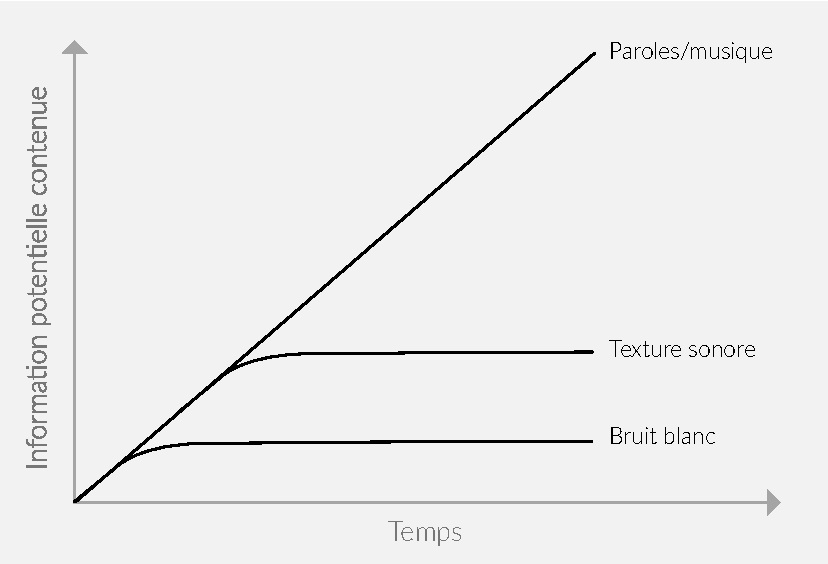
\includegraphics[width=\linewidth]{gfx/texture}
        \caption[Information potentielle contenue dans les séquences d'événements, les textures, et le bruit]{Information potentielle contenue dans les séquences d'événements, les textures, et le bruit. D'après \citep{saint1995classification}}\label{fig:texture}
\end{figure}

\subsubsection{Percevoir les textures}

Contrairement aux événements sonores, la texture est un objet simple, dont le traitement cognitif ne requière pas une analyse poussée. Ce point a été notamment prouvé par les travaux de Josh H. McDermott et ses co-auteurs \citep{mcdermott2011sound,mcdermott2013summary}. A l'aide d'un modèle de texture, inspiré du fonctionnement des premières étapes du système auditif humain allant de la cochlée jusqu'au thalamus, ils ont pu re-synthétisé des textures sonores en ne servant que de statistiques simples calculés à partir de représentations temps-fréquence de signaux de textures enregistrés. Dans un premier temps, la capacité des sujets à identifier les textures synthétisées a été testée \citep{mcdermott2011sound}. Les résultats ont montré que les sons de synthèse étaient aussi bien identifiés au les sons enregistrés, démontrant ainsi que les statistiques du signal sont utiles d'un point de vu cognitif à la reconnaissance, le cerveau étant capable de traiter des sons simples uniquement à partir de l'extraction de ces statistiques.

Dans une seconde expérience, \citep{mcdermott2013summary} les sujets ont dû reconnaître, parmi une triade de sons synthétisés, celui produit par une source différente (\ie un type de texture différent). Les résultats montrent que la capacité de discrimination est fonction de la durée des textures. Plus cette dernière est élevée, plus la capacité à discriminer est importante.  Ce résultat valide les hypothèses formulées par \citep{saint1995classification} sur l'existence d'une période d'attention, nécessaire au cerveau pour comprendre le stimuli comme une texture, et ainsi l'analyser sur la base de statistiques extraites.

\gl{Perception bruit blanc}

\subsubsection{Période d'attention}

Dans nos travaux nous nous sommes également penchés sur cette notion de période d'attention. En poussant cette vision composite à l’extrême, une texture peut être vu comme un empilement d’événements sonores qui cessent d'être perçus de manière distincte, dès lors que ces derniers forment un tout homogène et stable. 

Nous avons suivi cette idée afin de bâtir un protocole permettant de d'analyser la période d'attention. Nous faisons l'hypothèse qu'à partir du moment ou un événement peut être isoler d'un mixture d'événements du même type, le cerveau ne perçoit plus la mixture comme une texture, mais comme une succession d'événement.

Nous avons monté une expérience de reconnaissance de type oui/non (\Cf~\ref{app:xp_texture} pour une description exhaustive de l'expérience). Chaque stimuli est composé d'un son cible, suivi d'une séquence d'événement enchevêtrés de 6 secondes (\Cf~\ref{fig:xptexture}.a). L'objectif pour le sujet est d'indiquer si oui ou non il a entendu le son cible dans la séquence d’événements.

Les séquences sont des sons de trafic, simulés en agglomérant des sons isolés de voiture. La simulation est contrôlée par un paramètre réglant l'espacement temporel inter-onset moyen entre les événements. Cinq valeurs d'espacement sont considérées: $0.1$, $0.3$, $0.5$, $0.7$ et $0.9$ secondes. Les sons isolés de voiture ont tous une durée de $1$ seconde. Pour chaque espacement, nous simulons 20 séquences de trafics, chaque sujet devant alors écouter 100 stimuli. La moitié de ces stimuli sont des pièges, le son cible y étant absent. Nous mesurons les performances des sujets en utilisant la mesure de sensitivité $d'$ (\Cf~Figure~\ref{fig:xptexture}.b). Les résultats montrent que la mixture cesse d'être perçue comme une texture à partir d'un espacement de 0.42 secondes, soit la durée moyenne des événements utilisés (\Cf~Figure~\ref{fig:xptexture3}).

\begin{figure}[bth]
        \myfloatalign
        \subfloat[]
        {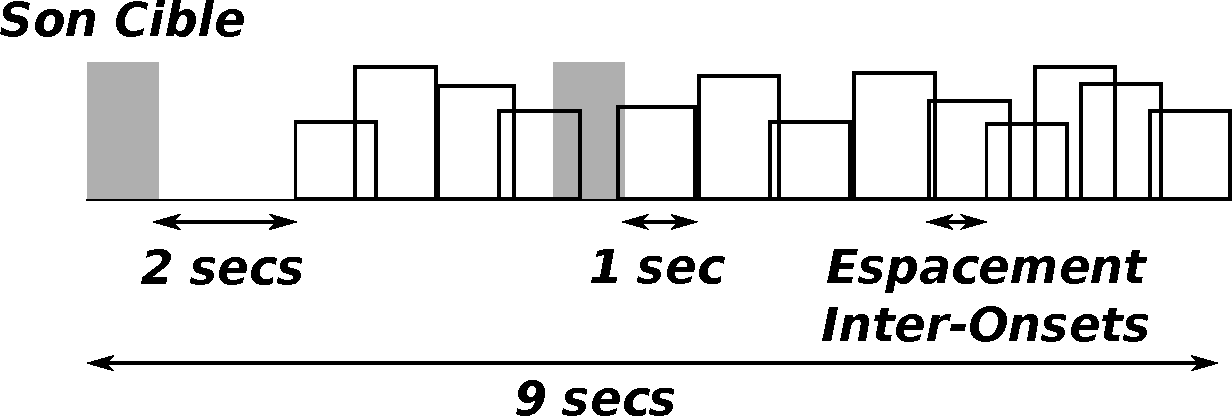
\includegraphics[width=.5\linewidth]{gfx/xpTexture1}}
        \subfloat[]
        {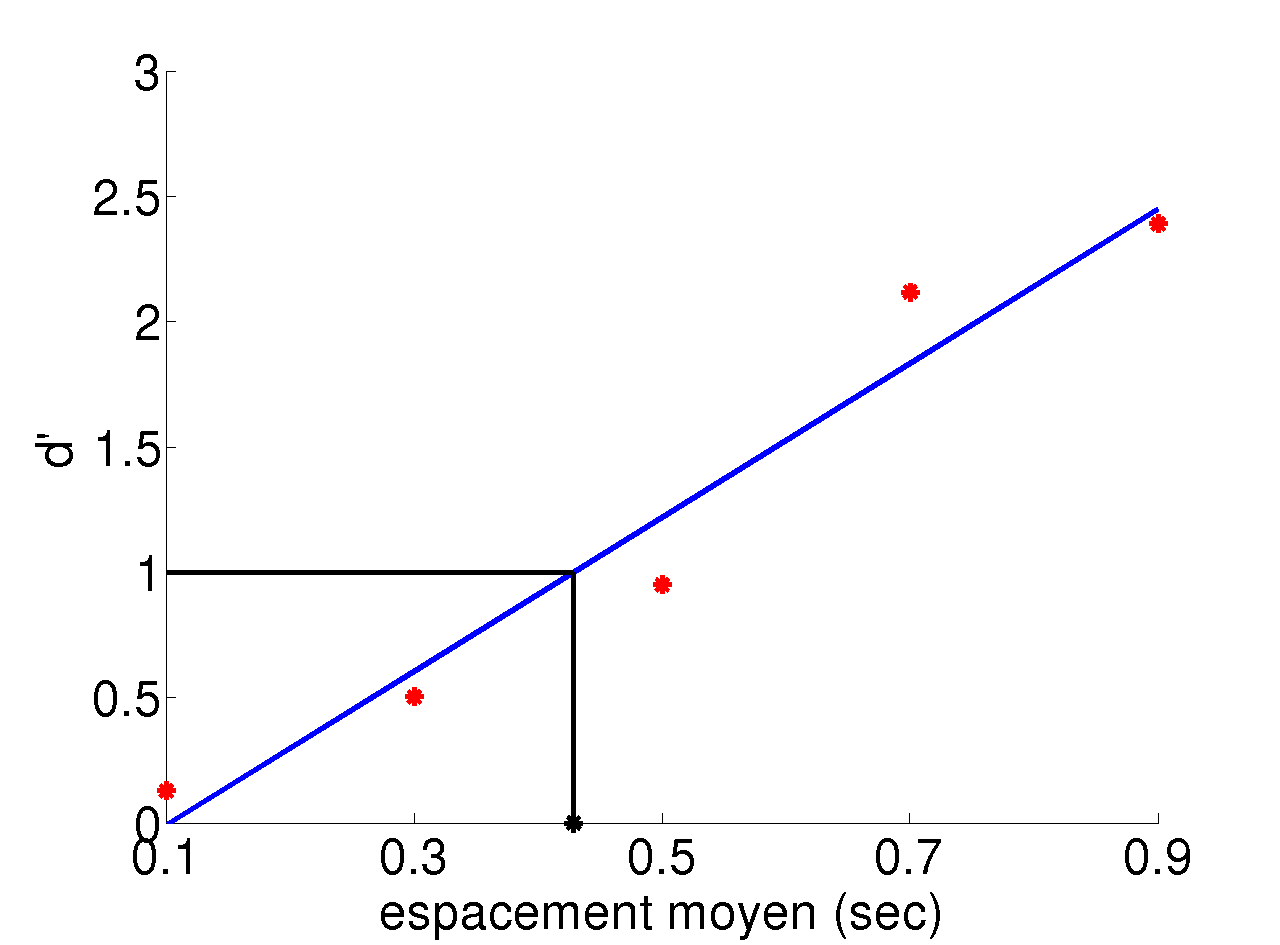
\includegraphics[width=.5\linewidth]{gfx/xpTexture3}}
        \caption[Experience sur la période d'attention]{Experience sur la période d'attention. (a) la nature des stimuli utilisés. (b) le seuil d'espacement moyen permettant de faire la distinction entre une séquence d'événements et une texture}\label{fig:xptexture}
\end{figure}


\subsubsection{Connexion}


Il est possible de faire des connexions entre les notions de textures/événements, et celles des scènes amorphes/événementielle mises en lumière par \citep{maffiolo_caracterisation_1999}. Pour la notion de texture, nous sommes très proches de celle des séquences amorphes
De même, on peut voir nos événements comme les objets composant les séquences événementielles. 

Cette dimension événement/texture est cependant orthogonale à celle de ``\,bruit de fond\,'' / ``\,événements de premier plan\,'' (\emph{background}/\emph{foreground}), utilisée dans le langage courant pour discriminer l’environnement urbain. Concernant les notions de background et de foreground, nous considérons que l'une et l'autre peuvent être vue comme des flux auditifs. Un flux auditif peut être composée de textures et d’événements regroupés dans le but de faciliter le traitement auditif de la scène. 

%*****************************************
%*****************************************
%*****************************************
%*****************************************
%*****************************************
